\chapter{Quantitative Genomic Comparisons of Embryogenesis Between Species do not Support a Generalized Phylotypic Stage}\thumbforchapter
\chaptermark{Quantitative Genomic Comparisons Between Species do not Support a Generalized Phylotypic Stage}
\chapterauthor{Maarten van der Sande, Gert Jan C. Veenstra, Simon J. van Heeringen}
\newpage

\section{Abstract}

The phylotypic stage is the period during embryonic development that is most conserved between species of the same phylum. Whereas evolutionary conservation in the phylotypic stage has historically been defined by qualitative morphological descriptions, more recently it has been explored and analyzed in the context of quantitative molecular similarity. Here we explore the concept of the molecular phylotypic stage in the context of comparative analyses, by focusing on the predictions of the different evolutionary developmental models. We argue that these models are not explicitly defined, and because of this ambiguity are unfalsifiable. As such we advocate for more explicit definitions and expectations of evolutionary developmental models and recommend the use of within-species, within-phylum, and between-phylum controls. We apply these controls to four recent molecular studies of the phylotypic stage and show that these analyses do not support the conclusions that are drawn from them. In our re-analyses, most between-species patterns seem to be caused by within-species effects. A notable exception is the inverse hourglass model, also known as the mid-developmental transition, which is caused by a statistical artifact of normalization. To our knowledge, there is no comparative molecular study that includes all three controls, and as such we see no molecular support for a well-defined phylotypic stage or its related hourglass and inverse hourglass models.

\section{Introduction}

Embryonic development is a complex and highly orchestrated process that begins with a single fertilized egg and culminates in the formation of a multicellular organism with a defined body plan and specialized organs. Even though both the eggs and adults of related species can be morphologically quite different, a seemingly remarkable period of similarity occurs in early development. This period of similarity is most easily observed for related species and is therefore known as the phylotypic stage (or period\cite{Richardson1995}). Over the years different models and explanations for its existence have been proposed\cite{Kalinka2012,Irie2014,Drost2017}.

The idea of a morphologically similar embryonic stage between related species dates back to Aristotle\cite{Aristotle1943}, but was formalized and popularized by Karl Ernst von Baer and Ernst Haeckel\cite{haeckel1866,baer1828}. In the early 1800s, von Baer formulated his four laws of embryology based on post-gastrulation embryos. His first law states that \textit{the more general characters of a large group appear earlier in the embryo than the more special characters}. This means that as an embryo develops, it first develops its oldest phylum-specific features, to then respectively develop its class, order, family, and species-specific features. Simply put, embryos of related species become increasingly diverse as development proceeds. Haeckel promoted a more radical view. Expanding on the work of Etienne Serres and Johann Friedrich Meckel, Haeckel related evolutionary history to developmental conservation in the recapitulation theory, popularized with the phrase \textit{ontogeny recapitulates phylogeny}. The recapitulation theory suggests that embryonic development is a replay of evolutionary history, where an embryo consecutively develops from adult stages of ancestral species to adult stages of descendants. In its strongest form, the recapitulation theory has been discredited, as development is not a repetition of evolution\cite{ehrlich1974}. Nonetheless, Haeckel's observations of similarities between embryos of different vertebrate classes, have, together with von Baers’ laws, formed the basis for the current models of evolutionary development (evo-devo).

The notion of similar embryonic stages between related species has led to two competing models of evolutionary development. The \say{funnel} or early-conservation model is closely linked to von Baer's first law, predicting the highest morphological similarity early in development. The hourglass model instead is based on the longstanding notion of a similar stage during mid-embryogenesis\cite{His1875}, but the first to describe it as an hourglass was Paul Medawar in 1954\cite{Medawar1954}. Medawar argues that somewhere mid-embryogenesis is the most morphologically conserved stage for vertebrates. This stage corresponds to Haeckel's phylotypic stage, but different from Haeckel's recapitulation theory, different species are thought to be more diverse both before and after the mid-embryogenesis state. More recently, these ideas have been examined with molecular genomic data, leading to a generalization of the hourglass model across phyla and kingdoms (insects\cite{Kalinka2010}, plants\cite{Quint2012} and fungi\cite{Cheng2015}), where each phylum now is expected to have its separate stage of maximum similarity during mid-embryogenesis. The phylotypic stage, initially called the \textit{phyletic stage}, refers to the point of maximum similarity in these models\cite{Cohen1963, Seidel1960}. More recently an inverse hourglass model has been proposed for comparisons between phyla, where specifically the beginning and end of embryonic development seem conserved, and the least molecular similarity is seen at the phylotypic stage\cite{Levin2016}.

Whereas the phylotypic stage has originally been defined based purely on qualitative morphological descriptions alone, the definition has recently been interpreted in terms of conserved patterns of gene expression. A popular addition is the idea that HOX genes are the master regulators of the phylotypic stage for vertebrate development\cite{Duboule1994}. Moreover, similarity in specific morphological features has been generalized to mean similarity across all genes or genomic features such as regulatory elements. These quantitative comparisons can roughly be divided into two distinct methodological approaches; (i) calculating a conservation metric for a single time series for each time point, where conservation metrics include the average evolutionary age of transcripts\cite{DomazetLoso2010}, the gene mutation rate index\cite{Quint2012, Piasecka2013}, embryonic lethality\cite{Uchida2018}, the relationship between timing of DNA accessibility and its evolutionary age\cite{Uesaka2019}, and the variance between replicates\cite{Liu2020, Uchida2022}. These results are usually visualized as a line graph where the x-axis represents embryonic development, and the y-axis the conservation metric. The second approach (ii) compares orthologous features between time points of two different species directly. Orthologous features that have been compared are cell type proportions\cite{Mayshar2023}, gene expression similarity\cite{Irie2011, Kalinka2010, Levin2016, marletaz2018, PerezPosada2022, Leong2021}, and regulatory DNA accessibility similarity\cite{Hu2017, Liu2021}. The comparison between two time-series is usually visualized as a heat map, where each axis represents the embryonic development of a species, and the color represents (dis)similarity (Fig. \ref{fig:models}). Both of these quantitative approaches have been used to study the phylotypic stage, but the second approach, comparing two time-series directly, is the focus of this study. 

\begin{figure}[H]
    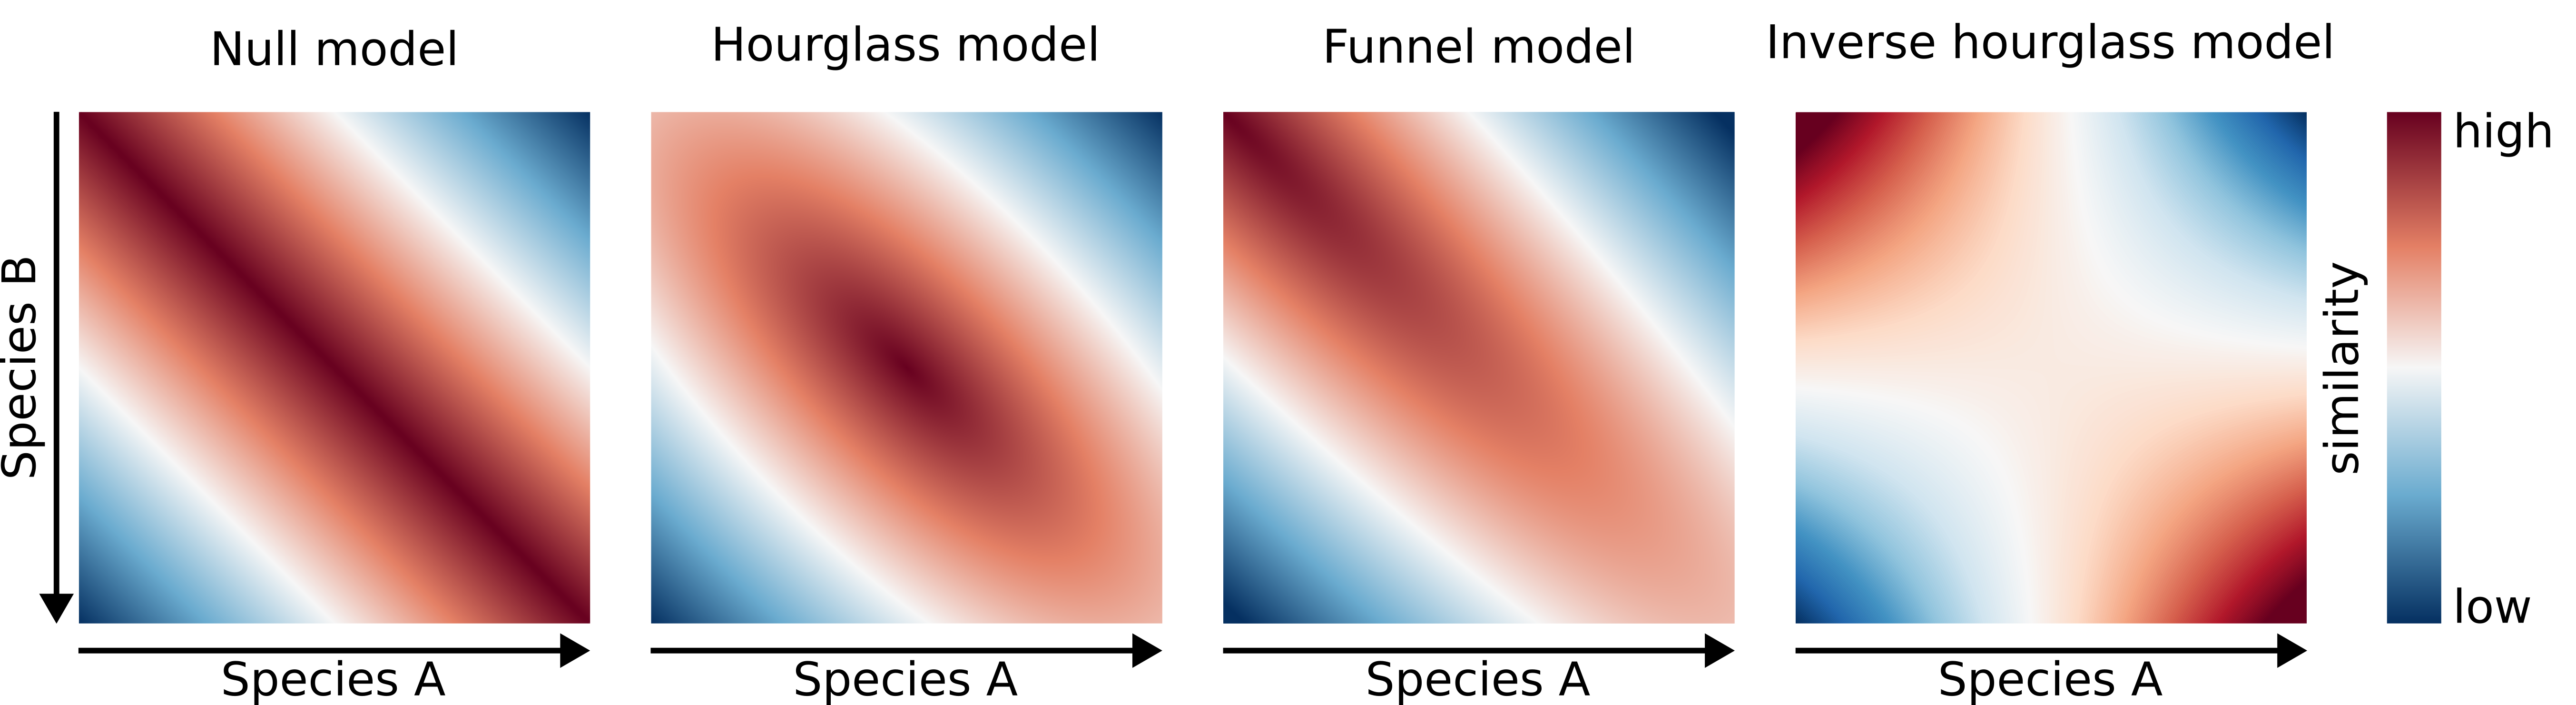
\includegraphics[width=\linewidth]{ch.hourglass/images/models.png}
    \caption{\textbf{Examples of developmental similarity along embryonic development for different comparative models}. These figures are usually ordered from top-left to bottom-right, where the x-axis represents embryonic development for species A, and the y-axis represents embryonic development for species B. The null model represents the case where there is no developmental stage of higher or lower similarity between the two species. The hourglass model predicts a point of maximum similarity somewhere mid-embryogenesis for species of the same phylum, and the funnel model instead predicts the highest similarity at the start of embryonic development. Finally, the inverse hourglass model predicts that for comparisons between-phyla, a point exists in mid-development that is the least conserved.}
    \label{fig:models}
\end{figure}

While quantitative studies are seen as offering an unbiased approach to studying the phylotypic stage, their results can be influenced by experimental design, including the analysis of the data. This, in turn, highlights the importance of incorporating appropriate controls. To give some examples; based on morphological timings, both an hourglass\cite{Cordero2020} and an inverse hourglass\cite{OlafRP2003} have been found. Based on RNA-seq data, Chan \textit{et al.} found an hourglass pattern, but with an identical analysis on microarray data, they found no temporal conservation pattern\cite{Chan2021}. Piasecka \textit{et al.} find that the observed conservation pattern is highly dependent on the metric used. In their work, genes are split into groups based on their maximum expression. There is no difference between the groups based on the $d_n / d_s$-ratio. Gene duplications and new gene introductions are least occurring in early conservation, but genes expressed in mid-development have the most highly conserved non-coding elements. However, all gene-based properties coherently show the least conservation for the latest stages\cite{Piasecka2013}. Moreover, Piasecka \textit{et al.} show that a popular similarity metric, the transcriptomic age index\cite{DomazetLoso2010}, expresses completely different conservation patterns based on whether or not the data has been log-transformed\cite{Piasecka2013}. Finally, Levin \textit{et al.} describe a universal between-phyla inverse hourglass \cite{Levin2016}, whilst Perez-Posada \textit{et al.} with a similar methodology instead report an hourglass for their comparison between deuterostomes and the chordate amphioxus\cite{PerezPosada2022}. Moreover, in an independent re-analysis of the work of Levin \textit{et al.}, their inverse hourglass was found not to be statistically significant\cite{Dunn2018}. 

The dependence on experimental design when studying the phylotypic stage is problematic and highlights the need for elaborate controls and clearly defined expectations. The phylotypic stage, the hourglass model, and the funnel model, however, do not pose explicit expectations on the similarity of embryos from different phyla. Yet, as the word phylotypic is a compound word of phylum and typical, it is suggestive of features conserved within a phylum but not between phyla. This implies that the point of maximum (molecular) similarity between phyla does not coincide with the phylotypic stages of the phyla involved. Levin \textit{et al.}\cite{Levin2016} use this implication in their inverse hourglass model as a new definition to distinguish phyla, where they note that embryonic dissimilarity is largest between species from different phyla at their respective phylotypic stages. Is it thus safe to assume that the point of maximum similarity between species from different phyla does not occur at their respective phylotypic stages? Similarly, what is expected if we were to compare the embryonic development of a species against itself? Transcriptomic variance between replicates, for instance, is lowest mid-development (Fig. \ref{fig:within_timepoint}), something that is used as an argument for the hourglass model\cite{Liu2020, Uchida2022}. The reasoning here is that gene regulation is most tightly regulated mid-development and that this translates to low transcriptomic variance between replicates. However, this changing variance over time can affect the similarity for direct comparisons between species. This begs the question of whether high similarity between species is an effect of a high similarity within species. Or would we expect that the phylotypic stage has a higher similarity between species of the same phylum even when corrected for within-species variance?

To address these ambiguities in the description of the phylotypic stage we have re-analyzed four recent molecular studies. By explicitly testing the within-species, within-phylum, and between-phyla assumptions about the phylotypic stage in these studies, we expose crucial flaws in the interpretation of the results from these analyses.

\section{Results}

\subsection{The phylotypic stage between zebrafish and frog is a superimposition of within-species effects} \label{subsection:marletaz}

In the paper \textit{Amphioxus functional genomics and the origins of vertebrate gene regulation}\cite{marletaz2018} Marl\'etaz \textit{et al.} investigated the similarity of orthologous gene expression in several chordates (\textit{Branchiostoma lanceolatum}, \textit{Danio rerio}, \textit{Gallus gallus}, \textit{Oryzias latipes}, and \textit{Xenopus tropicalis}), and consistently find a point of maximum similarity during mid-embryogenesis, in support of the hourglass model. All comparisons are within the same chordate phylum, but between-phyla or within-species comparisons are missing. In our re-analysis, we focus specifically on the comparison between \textit{D. rerio} and \textit{X. tropicalis}. By analyzing the original data with a similar methodology, we reproduce their result of a point of maximum similarity mid-embryogenesis. Furthermore, we incorporate within-species controls by comparing the \textit{D. rerio} time series from our study with a similar time series of \textit{D. rerio} from a different study \cite{White2017}, and apply the same approach for \textit{X. tropicalis} using data from \cite{Hu2017}. We show that the point of maximum similarity between \textit{D. rerio} and \textit{X. tropicalis} corresponds to the point of maximum similarity within each species. Finally, the current analysis cannot distinguish within-species effects from between-species effects, and as such no hard claims can be made about temporal conservation between these species.

Figure \ref{fig:betweenexperiment}B shows the pairwise similarity between all sampled stages of \textit{Danio rerio} and \textit{Xenopus tropicalis}, where similarity is based on the Jensen-Shannon distance (JSD) of the gene counts (TPMs). The JSD is a distance metric where a high value means low similarity between distributions and vice versa. The JSD follows an hourglass pattern with the point of maximum similarity at 20 hours post-fertilization for \textit{Danio rerio} and at 30-32 hours post-fertilization for \textit{Xenopus tropicalis}, marked by a black star. Our result is visually similar to the comparison by Marl\'etaz \textit{et al.} and the actual point of maximum similarity is adjacent to theirs, marked by a black pentagon. Figure \ref{fig:betweenexperiment}A and C show the related within-species comparisons, where the time-series of \textit{X. tropicalis} and \textit{D. rerio} are compared to the time-series of independent studies\cite{Hu2017,White2017}. Both these within-species comparisons show an hourglass-like pattern, with their point of maximum similarity during mid-embryogenesis. Note how the points of maximum similarity within-species closely match with the points of maximum similarity between-species. Similarly, figure \ref{fig:withinexperiment} shows all the within-species comparisons against itself, where we find that there is a high self-similarity at the point of maximum similarity between species. 

\begin{figure}[H]
    \centering
    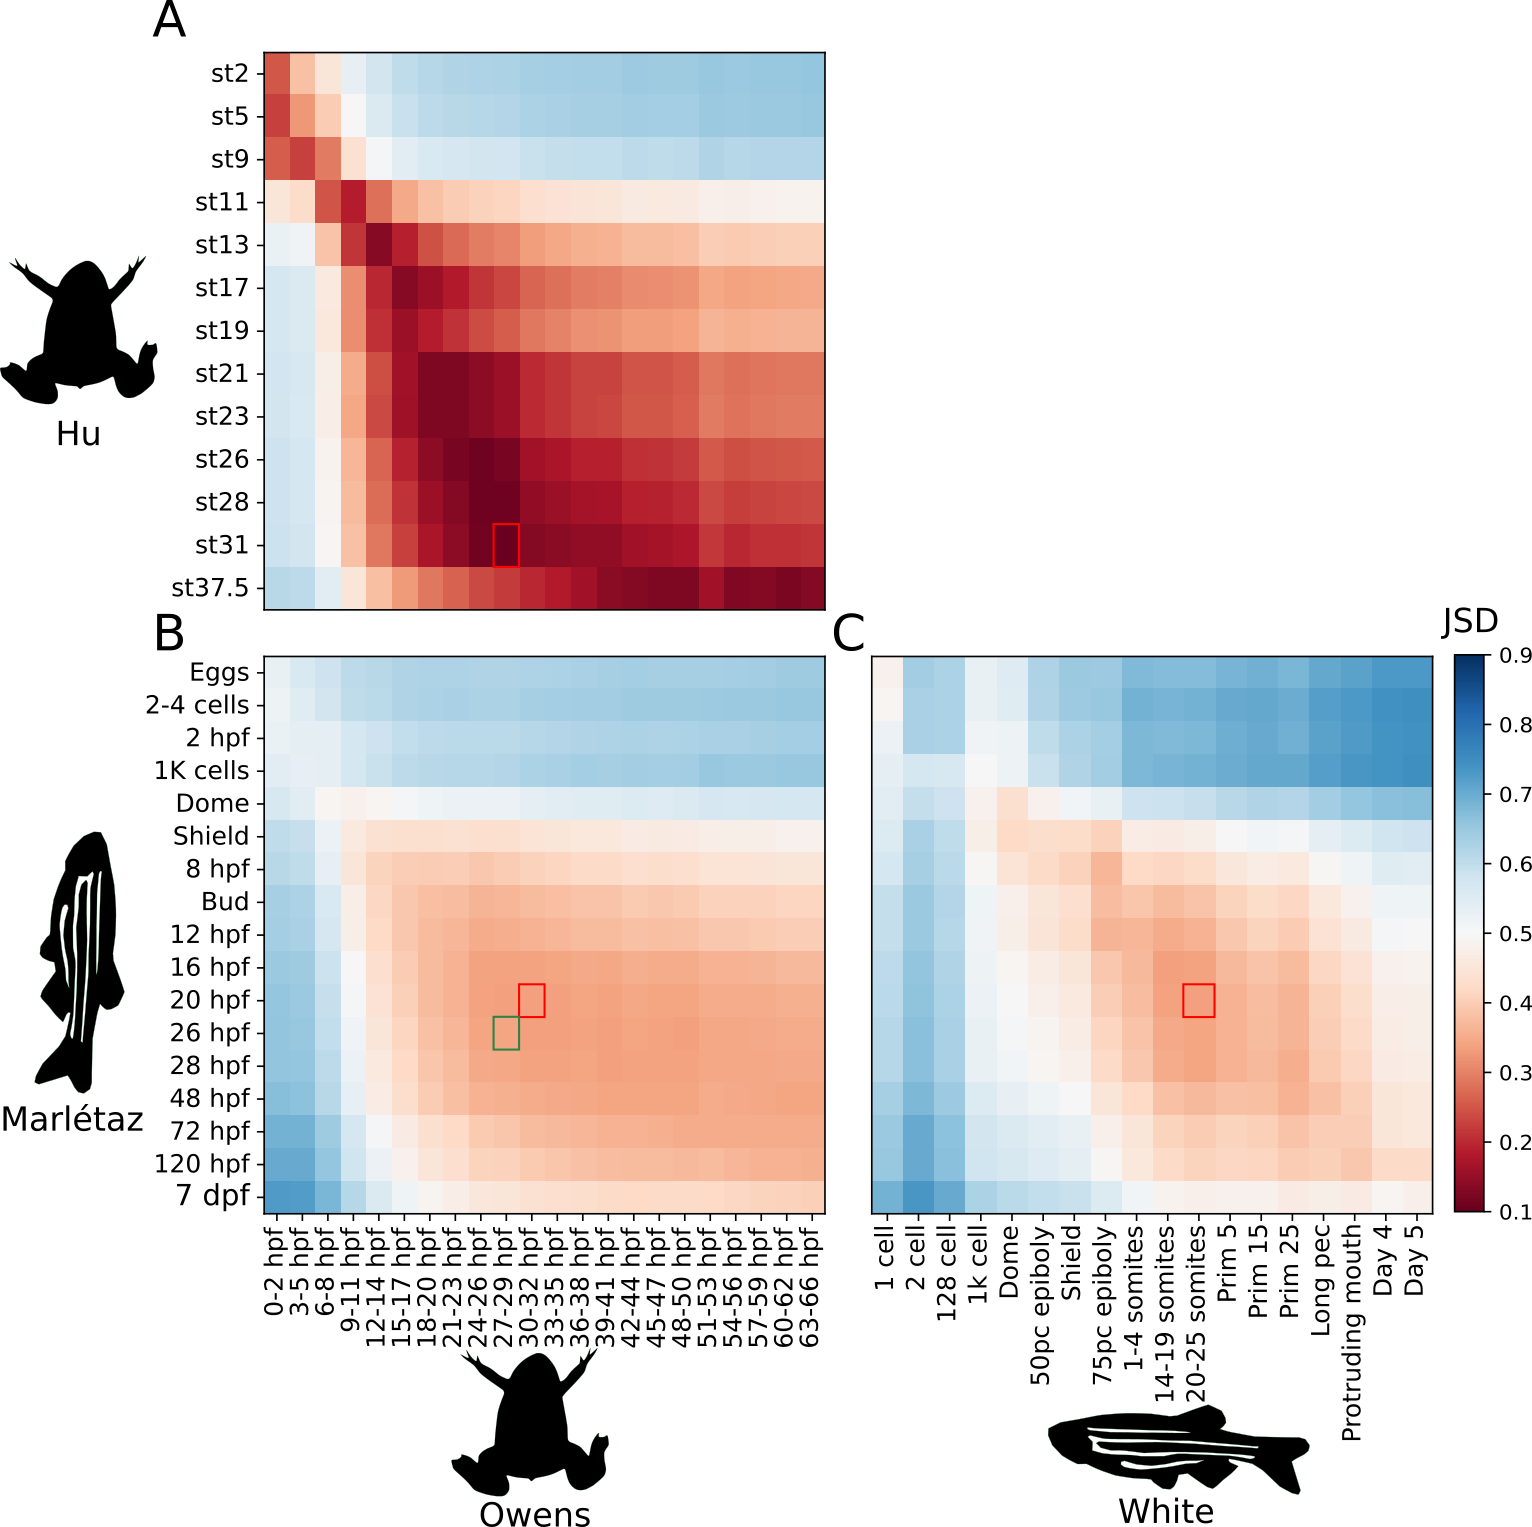
\includegraphics[width=0.8\linewidth]{ch.hourglass/images/between_experiment.png}
    \caption{\textbf{Within-species transcriptomic similarities translate to between-species transcriptomic similarities}. The heatmap of pairwise Jensen-Shannon distances between \textbf{(A)} two \textit{Xenopus tropicalis} time series, \textbf{(B)} \textit{Xenopus tropicalis} and \textit{Danio rerio}, and \textbf{(C)} two \textit{Danio rerio} time series. The point of lowest Jensen-Shannon distance is marked in each comparison by a black star, and the black pentagon represents the point of maximum similarity between \textit{Xenopus tropicalis} and \textit{Danio rerio} in the original study by Marl\'etaz et al.\cite{marletaz2018}. The between-species comparison appears to be a superimposition of the within-species effects.}
    \label{fig:betweenexperiment}
\end{figure}

Our re-analysis reveals that an hourglass pattern is already present when comparing the transcriptomes of \textit{D. rerio} and \textit{X. tropicalis} from different studies within each species independently. Consequently, any additional comparison made between such time series is susceptible to this effect. Based on our re-analysis, the between-species comparison can be explained as a combination of the two within-species patterns alone. It is still possible that even when correcting for within-species effects, the similarity between \textit{D. rerio} and \textit{X. tropicalis}  is highest at the phylotypic stage. However, without explicitly correcting for the within-species effects we cannot definitively determine whether certain embryonic stages are more or less conserved between species

\subsection{The mid-developmental transition is a statistical artifact of gene standardization} \label{subsection:levin}

In the paper \textit{The mid-developmental transition and the evolution of animal body plans}\cite{Levin2016} Levin \textit{et al.} compared the correlation coefficient of the expression of orthologous genes over time between ten species from different phyla. They found that most species-species comparisons display an inverse hourglass, with a high similarity early and late during development, but a period of low similarity mid-development. They refer to this period as the \textit{mid-developmental transition}. They note that the mid-developmental transition between phyla seems to correspond with each species' phylotypic stage. They then suggest that this pattern could be used to distinguish different phyla. In this re-analysis, we reproduce the finding of a between-phyla inverse hourglass. As suggested by Hejnol \textit{et al.}\cite{hejnol2016} we include a within-phylum control and show that this comparison also produces an inverse hourglass. Finally, we show that the inverse hourglass is a statistical artifact of standardization, and can not be used to infer temporal conservational patterns.

Figure \ref{fig:within_phylum}A shows the pairwise Pearson correlation coefficient of one-to-one orthologs between each developmental stage of \textit{Drosophila melanogaster} and \textit{Danio rerio}. With the same methodology as the original study, we get a dual-phase pattern where both the early and the late stages between the two species seem conserved, but with a period of low conservation in the middle. If we now apply the same methodology to the chordates \textit{D. rerio} and \textit{X. tropicalis} of the previous section, we get a similar biphasic pattern. Note that figure \ref{fig:within_phylum}B is based on the same sequencing data as figure \ref{fig:betweenexperiment}B. The main difference in processing between those is the inclusion of gene standardization (z-score).

\begin{figure}[H]
    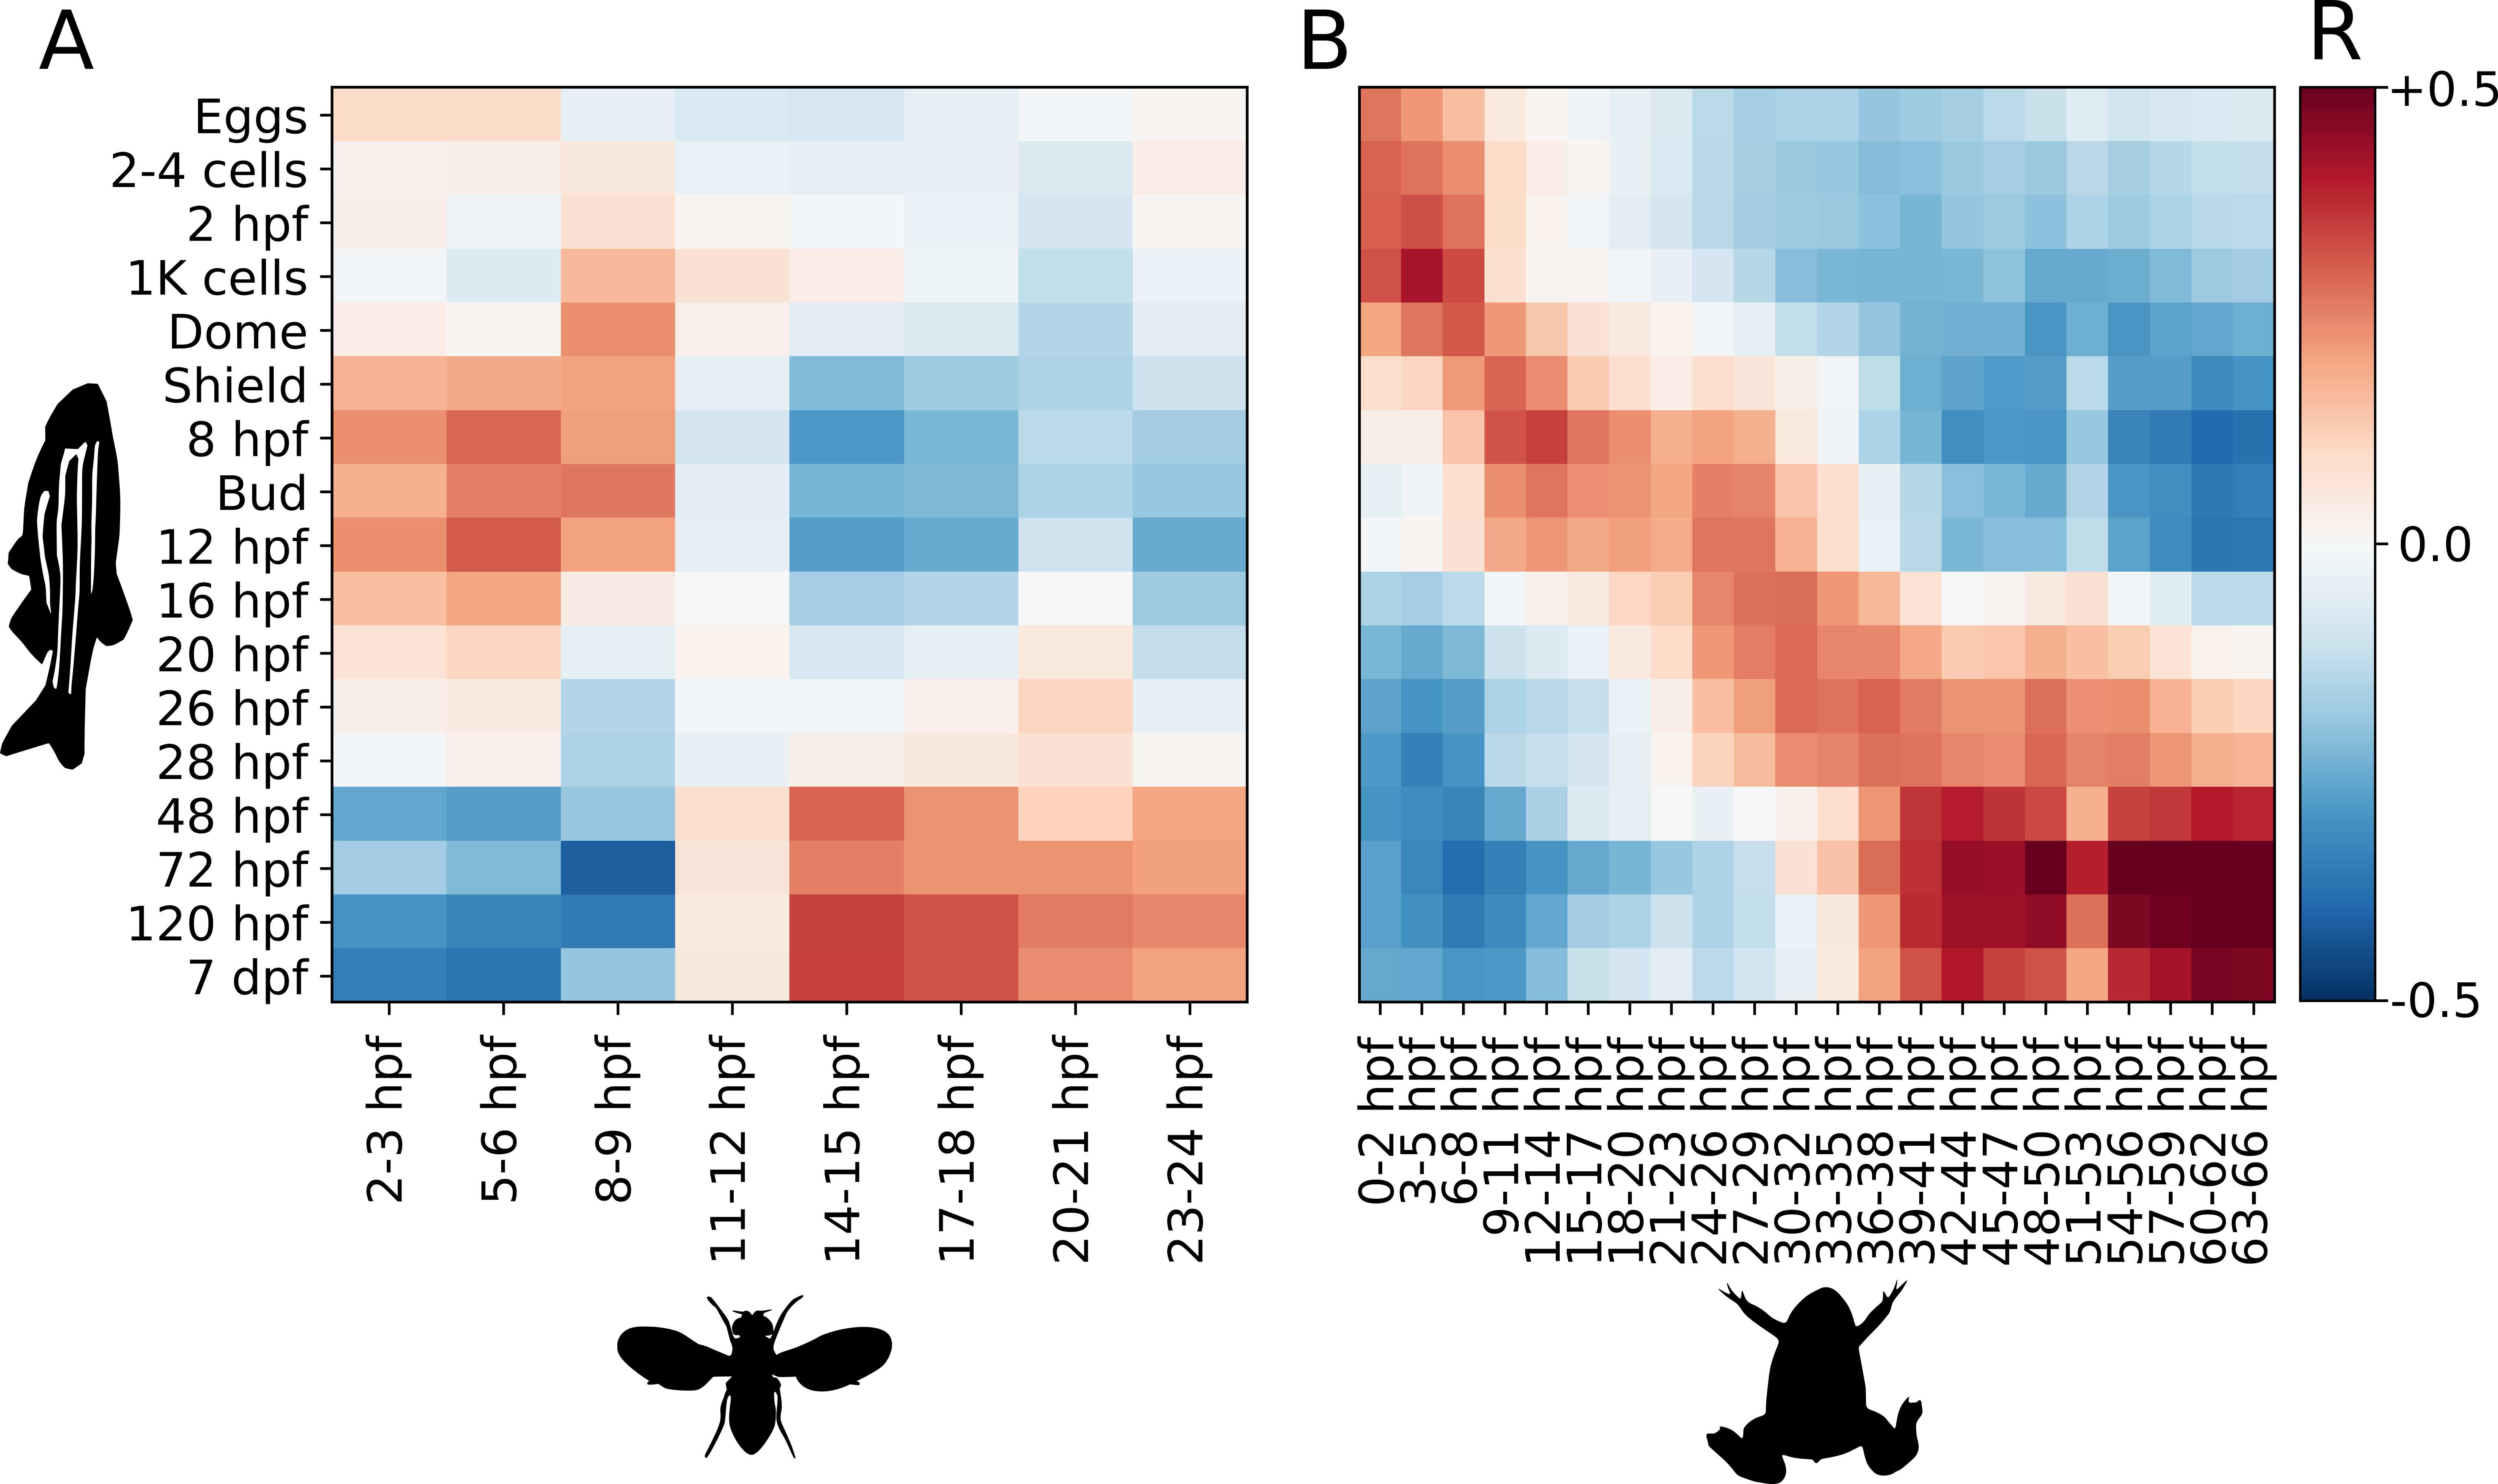
\includegraphics[width=\linewidth]{ch.hourglass/images/within_between_phyla.png}
    \caption{\textbf{The inverse hourglass is not exclusive to between-phyla comparisons}. Heatmaps of pairwise Pearson correlation coefficients \textbf{(A)} for a between phylum comparison of \textit{Danio rerio} and \textit{Drosophila melanogaster}, and \textbf{(B)} a within phylum comparison of \textit{Danio rerio} and \textit{Xenopus tropicalis}. A mid-developmental transition is visible for both comparisons.}
    \label{fig:within_phylum}
\end{figure}

Levin \textit{et al.} apply gene standardization, which involves subtracting the mean and dividing by the standard deviation over time for each gene. Standardization is generally a good practice for parametric methods like the Pearson correlation coefficient. In the case of gene expression data, standardization effectively scales each gene to have equal weight in the correlation coefficient. The use of standardization here leads to an unexpected side effect. In the absence of standardization, the data exhibits an hourglass-like pattern (see Fig. \ref{fig:standardization}A). However, after applying standardization, the pattern transforms into an inverse-hourglass shape. Even more surprising, we can cut each time series into four equal parts, and after standardization, three out of four comparisons still display a mid-developmental transition (Fig. \ref{fig:standardization}B). 

\begin{figure}[H]
    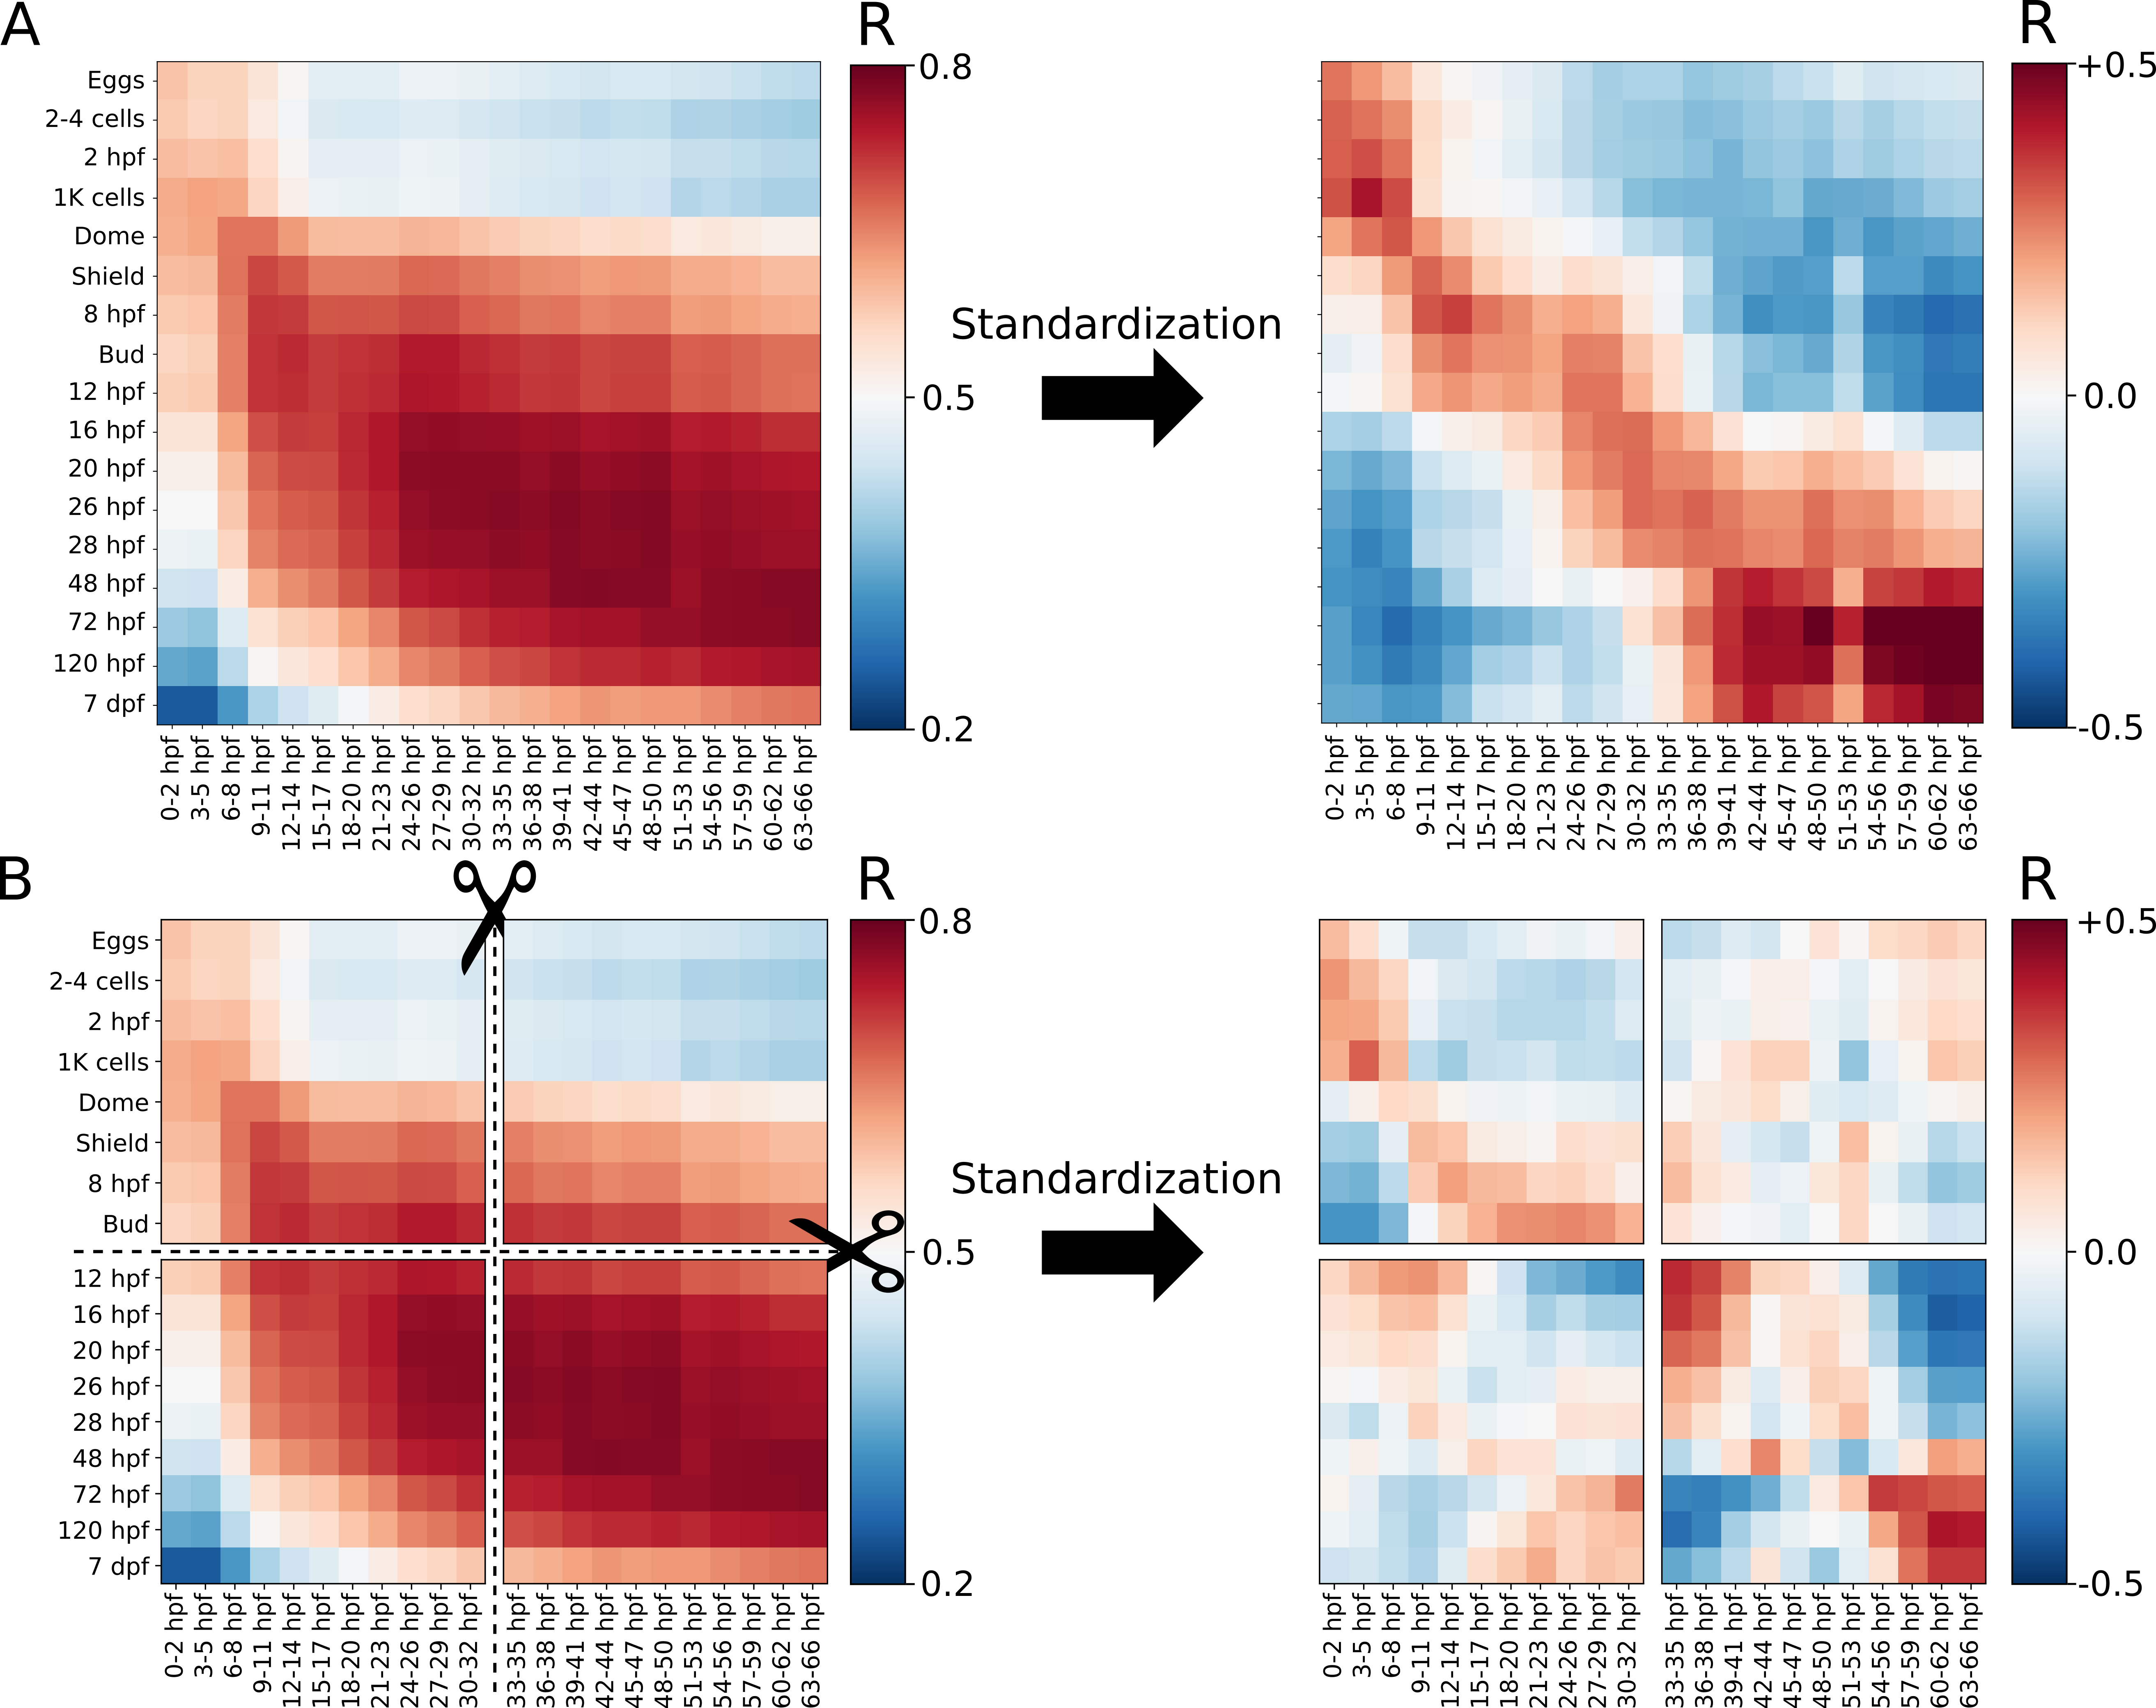
\includegraphics[width=\linewidth]{ch.hourglass/images/normalisation.png}
    \caption{\textbf{The inverse hourglass is a statistical artefact of gene standardization}. \textbf{(A)} shows the effect of standardization. Before standardization, an hourglass-like pattern is visible, whereas after standardization an inverse hourglass is visible. \textbf{(B)} shows the effect of standardization after dividing the time series into four equal parts. After standardizing each part, three out of four subsets now display an inverse hourglass. }
    \label{fig:standardization}
\end{figure}

To get an understanding as to why this happens we need to study the patterns of gene expression during development. Levin \textit{et al.} introduced the concept of a gene landscape, which offers a way to visualize gene expression patterns. The gene landscape is a histogram of the Pearson correlation coefficient for each gene with a linearly increasing line. A coefficient of 1 means that a gene is linearly going up over time, a coefficient of -1 means that a gene is linearly going down over time, and a coefficient of 0 means that a gene shows no linear temporal pattern. In figure \ref{fig:genelandscape} we show the gene landscape for \textit{D. rerio}, \textit{D. melanogaster}, and \textit{X. tropicalis}. For each gene landscape, we observe a bimodal distribution, with an enrichment for genes that are either going up or down in expression over time and relatively few genes having no (linear) temporal pattern. The scatterplot that Levin \textit{et al.} report (Extended Data Figure 5\cite{Levin2016}), unfortunately, hides this pattern, and a 2D histogram would have been a better choice. As embryos grow, one would expect practically all genes to increase in expression over time. But as RNA sequencing (without spike-ins) is inherently relative, genes are split into either one of two expression groups; a group where gene expression goes up or increases faster than the average gene (right side of the gene landscape) or the group where gene expression goes down or increases slower than the average gene (left side of the gene landscape). See figure \ref{fig:genelandscapenormalization} for the difference between per-embryo (spike-in) normalization and transcript per million (TPM) normalization for \textit{X. tropicalis} embryos.

\begin{figure}[H]
    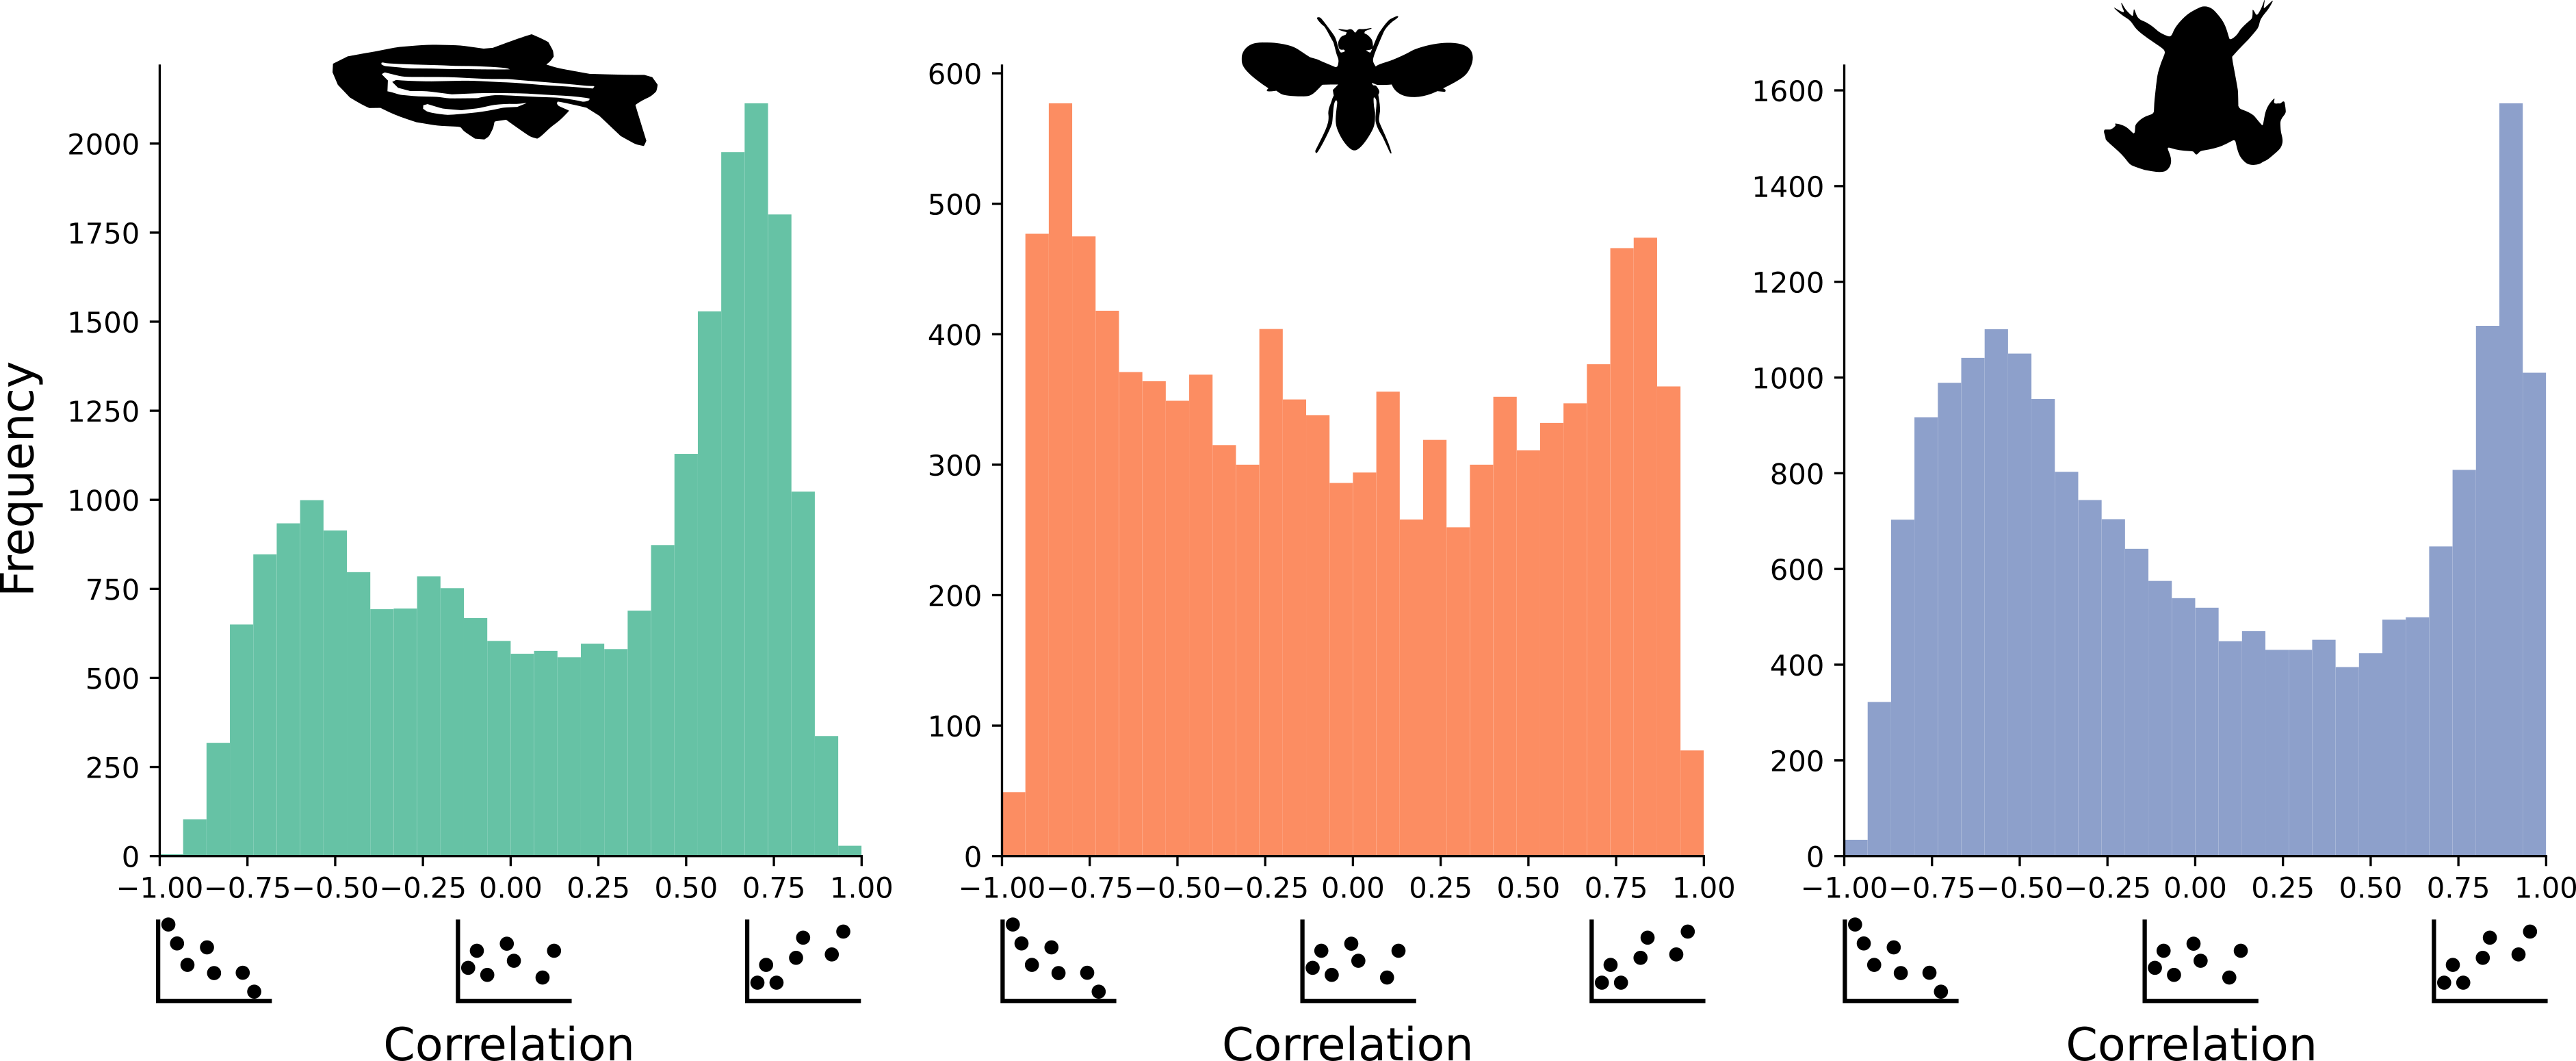
\includegraphics[width=\linewidth]{ch.hourglass/images/gene_landscape.png}
    \caption{\textbf{The gene landscape of \textit{D. rerio}, \textit{D. melanogaster}, and \textit{X. tropicalis} embryos}. The gene landscape is a histogram of the correlation coefficient of the expression of each gene with a linearly increasing line. Note how generally speaking there are two groups of genes; a group of genes that is upregulated, and a group that is downregulated during embryonic development.}
    \label{fig:genelandscape}
\end{figure}

Now that we understand that our genes can roughly be classified as either going up or going down over time, we can think about how this influences our analyses. To analyze the effects of the gene expression landscape on hourglass analyses, we simulated the time series of a single gene that has a binary expression profile, where at the start of our time series the gene is \textit{off}, and at a random time point switches \textit{on} and stays \textit{on} until the end of the series. We now imagine the expression profile of this gene in a related species and assume again that it starts \textit{off} and at a random time point switches \textit{on}. We can express the probability that these two imaginary time series are equal (section \ref{subsection:middevelopmenttransition}), and if we visualize these probabilities it is clear these odds display a mid-developmental transition (Fig. \ref{fig:inverse_math}). This theoretical derivation is however an oversimplification of what happens both biologically and methodologically and considers only a single gene. For this reason, we simulated two time series with continuous expression profiles. In these series half of the genes start in an \textit{off} state where expression is zero, and half in an \textit{on} state where expression is one. Similarly to the single-gene thought experiment, these genes, at a random time-point, gradually switch from \textit{off} to \textit{on}, or vice versa. We can now calculate the Pearson correlation coefficient between these simulated series, and we get a clear mid-developmental transition (Fig. \ref{fig:sim_explanation}). Similar to the biological data, if we cut the simulated data into halves, and apply standardization afterwards, we get a mid-developmental transition per subset of the data (Fig. \ref{fig:sim_normalisation}). 

By incorporating a within-phylum comparison it becomes clear that the mid-developmental transition is a statistical artifact of gene standardization. It can be considered a special case of Simpson's paradox, where by standardization gene expression gets put into two groups (high vs low expression). And even though there is no particular correlation within each group, there is a clear correlation when comparing the data set as a whole\cite{Saccenti2023}. This pattern is not caused by lowly expressed genes, as we applied the same criteria as Levin \textit{et al.} to only include dynamic genes (minimum expression of 10 TPM and at least a log2 fold change). We conclude that gene expression standardization in combination with the landscape of gene expression dynamics observed, produces the appearance of an inverse hourglass irrespective of the stages selected for analysis.

\begin{figure}[h]
    \center
    \includegraphics[width=0.8\linewidth]{ch.hourglass/images/sim_explanation.png}
    \caption{\textbf{The inverse hourglass is present in simulated data with no temporal conservation.} A schematic representation of the simulation of gene expression of two time series (A and B) on a continuous scale. Two groups of genes exist and are identical between the time series; upregulated (green) and downregulated (red) genes. The timing of up- and downregulation is completely random. When comparing such time series with themselves (A vs A) there is no temporal pattern (null model), however when comparing two such time series (A vs B) an inverse hourglass appears. }
    \label{fig:sim_explanation}
\end{figure}

\subsection{The mouse and rabbit cell type proportion bottleneck is a within-species effect} \label{subsection:mayshar}

In the paper \textit{Time-aligned hourglass gastrulation models in rabbit and mouse}\cite{Mayshar2023} Mayshar \textit{et al.} analyzed the similarity between developing rabbit and mouse embryos on a single-cell level. One of the comparisons they make is how the correlation of cell type proportions between rabbits and mice changes over time. They observe an \say{hourglass-like} bottleneck of cell type proportions pre-gastrulation. In this re-analysis, we reproduce the between-species cell type proportion bottleneck. Additionally, we compared the mouse and rabbit time series against themselves and discovered similar bottlenecks. This bottleneck is caused by the combination of a statistical artifact of new cell types appearing and an inappropriate temporal scale. It is unlikely that the bottleneck signifies an evolutionary-developmental effect between \textit{M. musculus} and \textit{O. cuniculus}.

Figure \ref{fig:cellproportions} shows the pairwise Pearson correlation coefficient between cell type proportions of developing \textit{M. musculus} and \textit{O. cuniculus}. Figure \ref{fig:cellproportions}B is the between-species comparison and shows the same result as the original paper. Mayshar \textit{et al.} describe this as a stereotypical pattern, where the beginning of development is aligned but not synchronized. This then leads to a bottleneck at approximately E7.5 followed by a more synchronized gastrulation process marked by cellular diversification. They conclude that around E7.5-E7.7, the narrowest point of the bottleneck, mouse and rabbit gastrulation are aligned with maximum specificity. However, when we compare the time series of \textit{O. cuniculus} against itself (a within-species comparison) we see a similar bottleneck (Fig. \ref{fig:cellproportions}C). Before E7.5 the rabbit embryo consists of a small number of cell types, forcing the cell type distributions into one of two groups; a group of cell types that do not occur, and a group of cell types that do occur. From E7.7 on, practically all cell types are present. All comparisons within \textit{O. cuniculus} before E7.5 give high correlation values because in this case, the Pearson correlation represents whether identical cell types are present. It says little about the correlation coefficient between cell types (known as Simpson's paradox \cite{Saccenti2023}). The bottleneck at E7.5 is caused by the rapid appearance of new cell types. Similar problems exist for the \textit{M. musculus} time series but are less pronounced. These within-species effects then get carried over to the comparison between \textit{M. musculus} and \textit{O. cuniculus}, leading to a deceptive between-species pattern.

\begin{figure}
    \center
    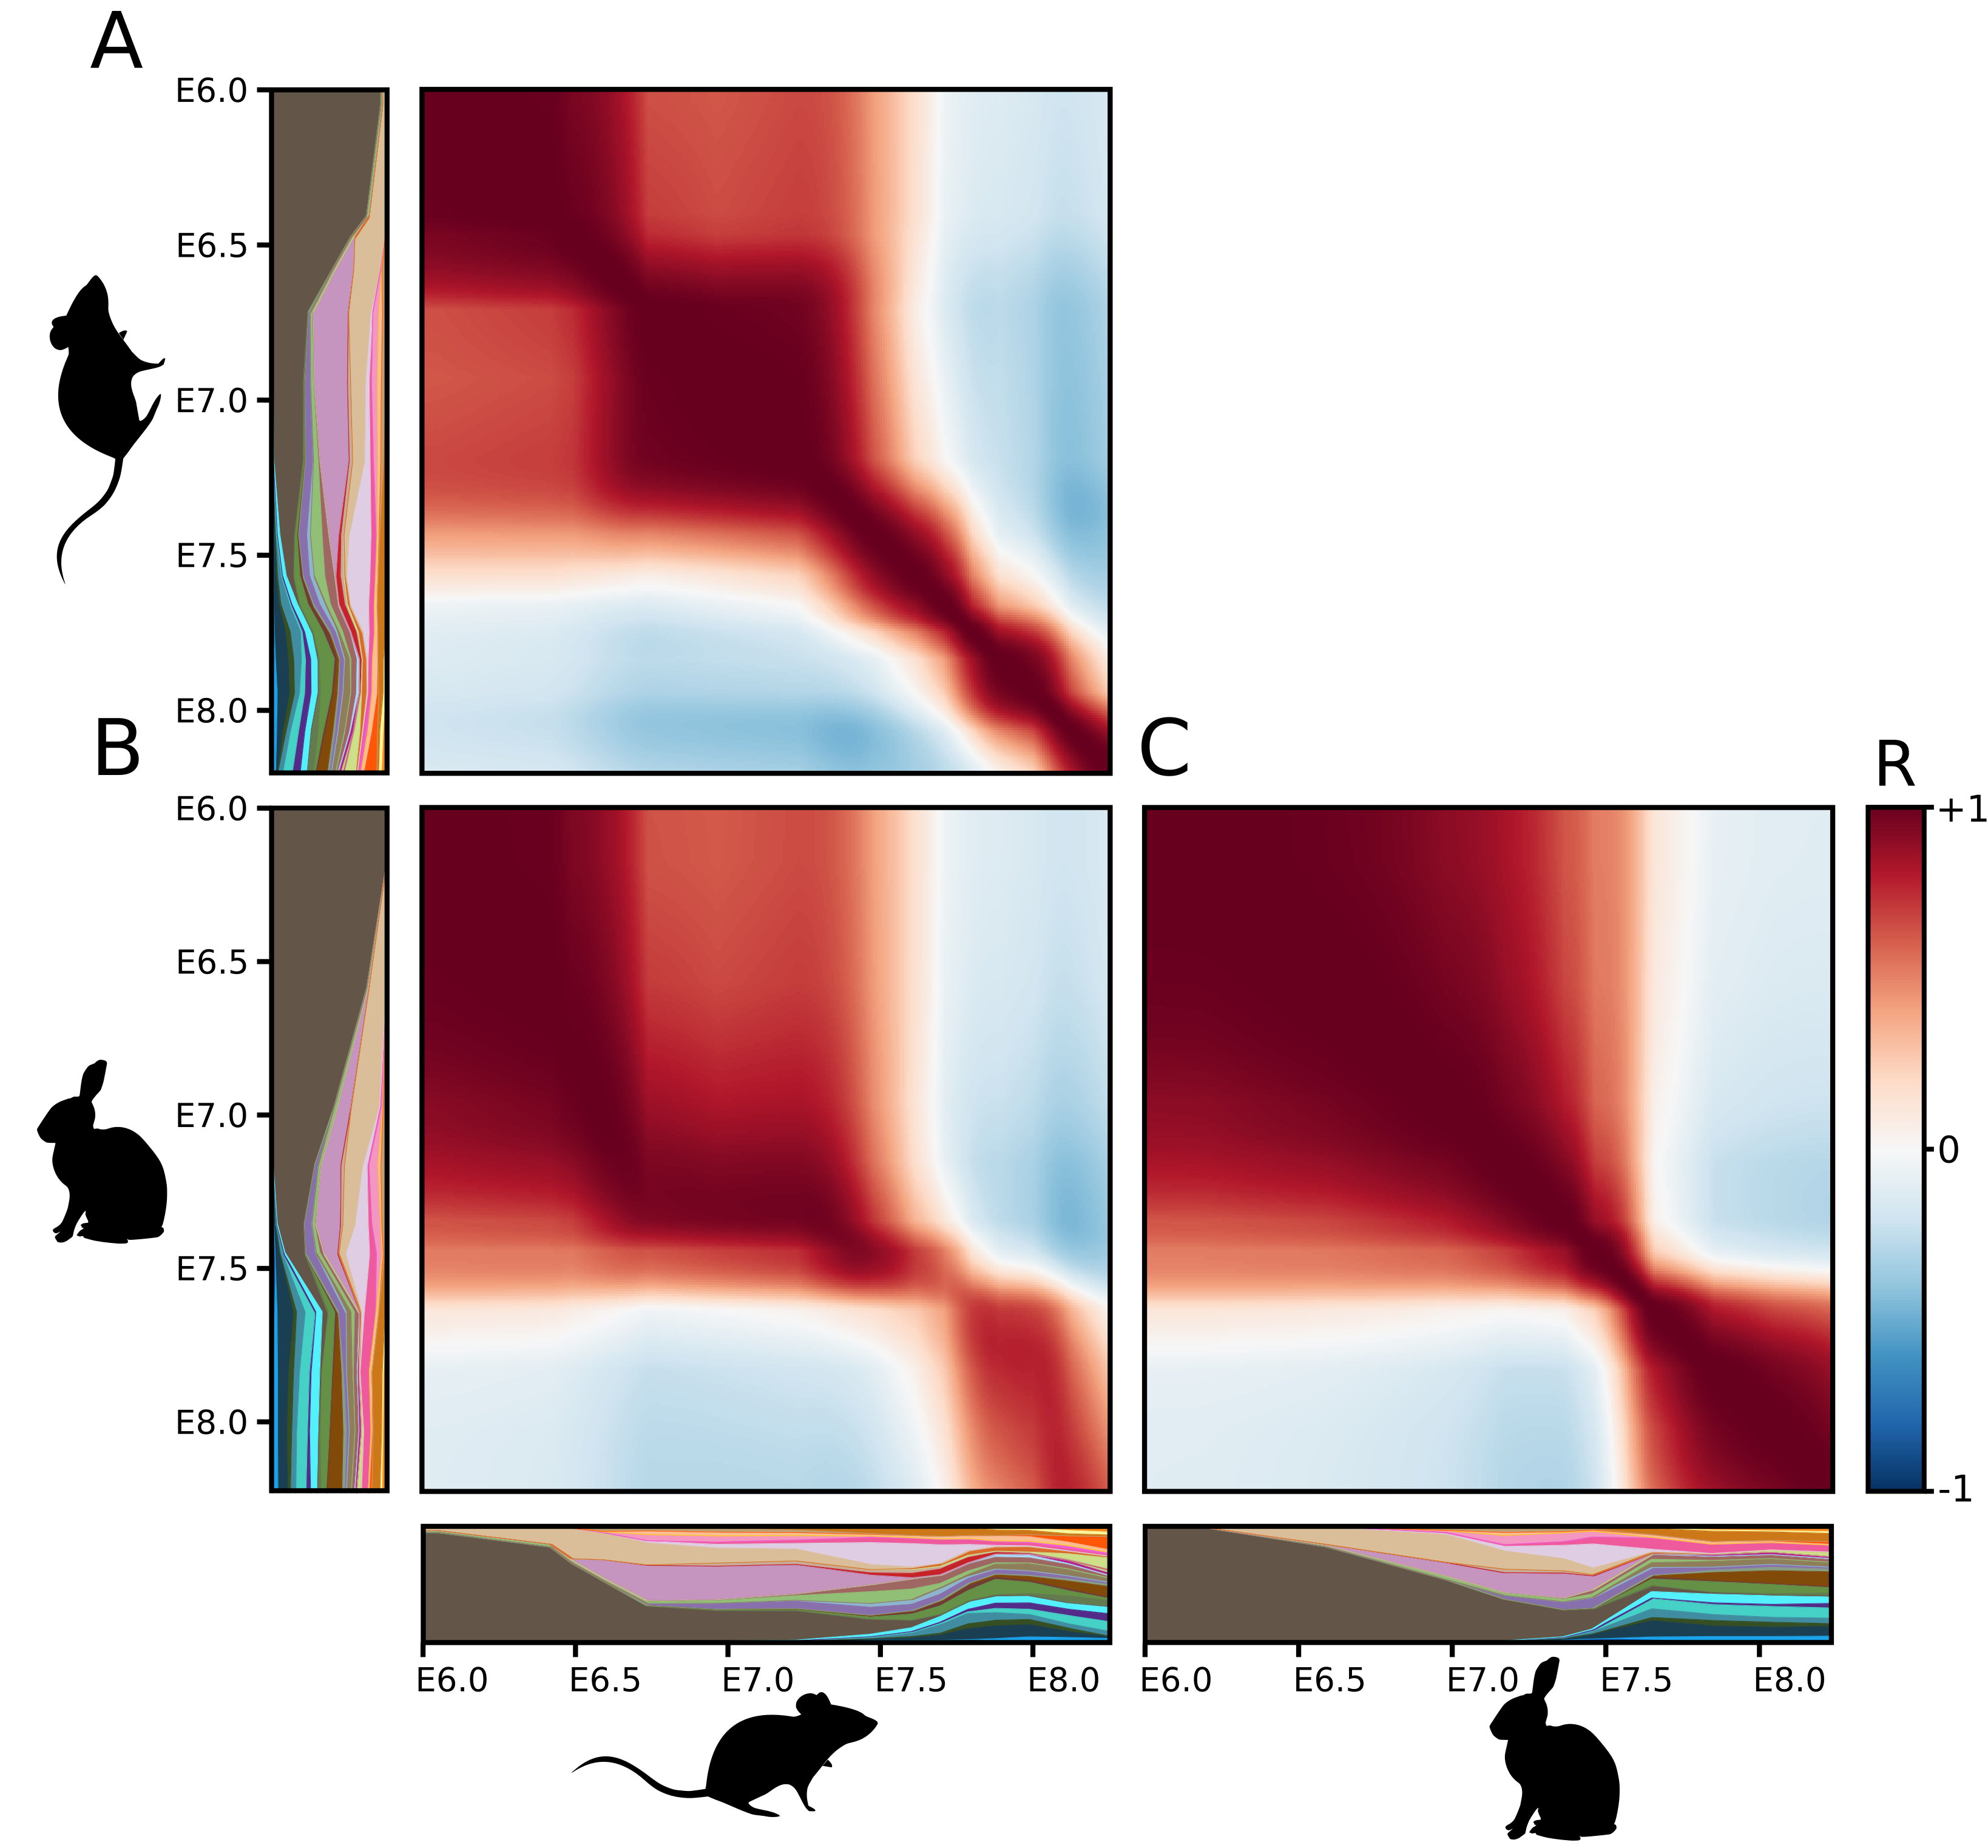
\includegraphics[width=0.8\linewidth]{ch.hourglass/images/mouse_rabbit_cellproportions.png}
    \caption{\textbf{Within-species cell type proportion similarities translate to between-species cell type proportion similarities}. Heatmap of pairwise Pearson correlation coefficients between \textbf{(A)} \textit{M. musculus} with itself, \textbf{(B)} \textit{M. musculus} and \textit{O. cuniculus}, and \textbf{(C)} \textit{O. cuniculus} with itself. The heatmaps are accompanied by cell-type proportion charts with similar coloring as the original paper. The between-species pattern seems to be a superimposition of the within-species effects.}
    \label{fig:cellproportions}
\end{figure}

What is surprising about this analysis is that the pattern that Mayshar \textit{et al.} describe as stereotypical pattern and hourglass-like, is neither stereotypical nor fits the hourglass model. For species of the same phylum, no such sudden changes in mid-development are expected. Instead, the opposite is predicted by the hourglass model. Moreover, the comparison in its current form displays a funnel pattern, with the highest similarity between \textit{M. musculus} and \textit{O. cuniculus} at the start of the time series which is gradually decreasing, although this is caused by global differences in cell proportions and does not represent a meaningful biological signal (Simpson's paradox). Furthermore, Mayshar \textit{et al.} conclude that their analysis shows that one can use absolute (linear) time for pairwise comparisons between gastrulating embryos. But considering the within-species comparisons, we can clearly see that the temporal axis is not representative of change. There is a higher rate of change happening between E7.5-E7.7 (5 hours) than between E6.0-E7.0 (24 hours). Altogether, the hourglass-like shape of temporal similarity between  \textit{M. musculus} and \textit{O. cuniculus} seems to be caused by within-species dynamics of cell type composition, which in turn is partially caused by unrepresentative temporal sampling and the fact that subgroups exist (Simpson's paradox).

\subsection{Temporal enhancer conservation between \textit{Drosophila} is confounded by the number of enhancers at each respective stage} \label{subsection:liu}

In the paper \textit{The hourglass model of evolutionary conservation during embryogenesis extends to developmental enhancers with signatures of positive selection}\cite{Liu2021} Liu \textit{et al.} compare the similarity of accessible regions over five matched embryonic developmental time points between two \textit{Drosophila} species (\textit{D. melanogaster} and \textit{D. virilis}). Liu \textit{et al.} find that the middle time point (TP3, 8-10 hours after egg laying) has the highest number of enhancers accessible, and that at TP3 \textit{D. virilis} and \textit{D. melanogaster} have the highest fraction of shared enhancers. TP3 coincides with the \textit{Drosophila} phylotypic stage, and thus this result is seen as supportive for the hourglass model. In this re-analysis, we show that this high conservation of enhancers at the phylotypic stage is explained by a different number of enhancers found per time point, and is not an evolutionary-developmental pattern.

In this study, conservation is estimated by the similarity between time point-specific enhancers between \textit{D. melanogaster} and \textit{D. virilis}, where time point-specific enhancers are defined as enhancers that are accessible in only one time point (TP). Enhancers are defined as accessible regions farther than 500 bp from a transcription start site. Finally, the similarity between the two species is calculated by dividing the number of TP-specific enhancers overlapping between both species by the total number of TP-specific enhancers for both species (Jaccard index). For all \textit{D. virilis} TP-specific enhancers, we inferred their corresponding orthologous regions in the \textit{D. melanogaster} with pslMap, restricting to one-to-one orthologs. Figure \ref{fig:peak_between}A shows the conservation over time between \textit{D. melanogaster} and \textit{D. virilis}, with the highest conservation at TP3, closely matching the results of Liu \textit{et al}. Figure \ref{fig:peak_between}B shows the number of  TP-specific enhancers per time point. The high amount of TP-specific enhancers at TP1 and TP5 can be explained by the fact that they are respectively the start and end of the time series. The high number of TP-specific enhancers at TP3, however, is not easily explained and in turn, raises the question of whether this can explain the high similarity between \textit{D. melanogaster} and \textit{D. virilis}.

\begin{figure}
    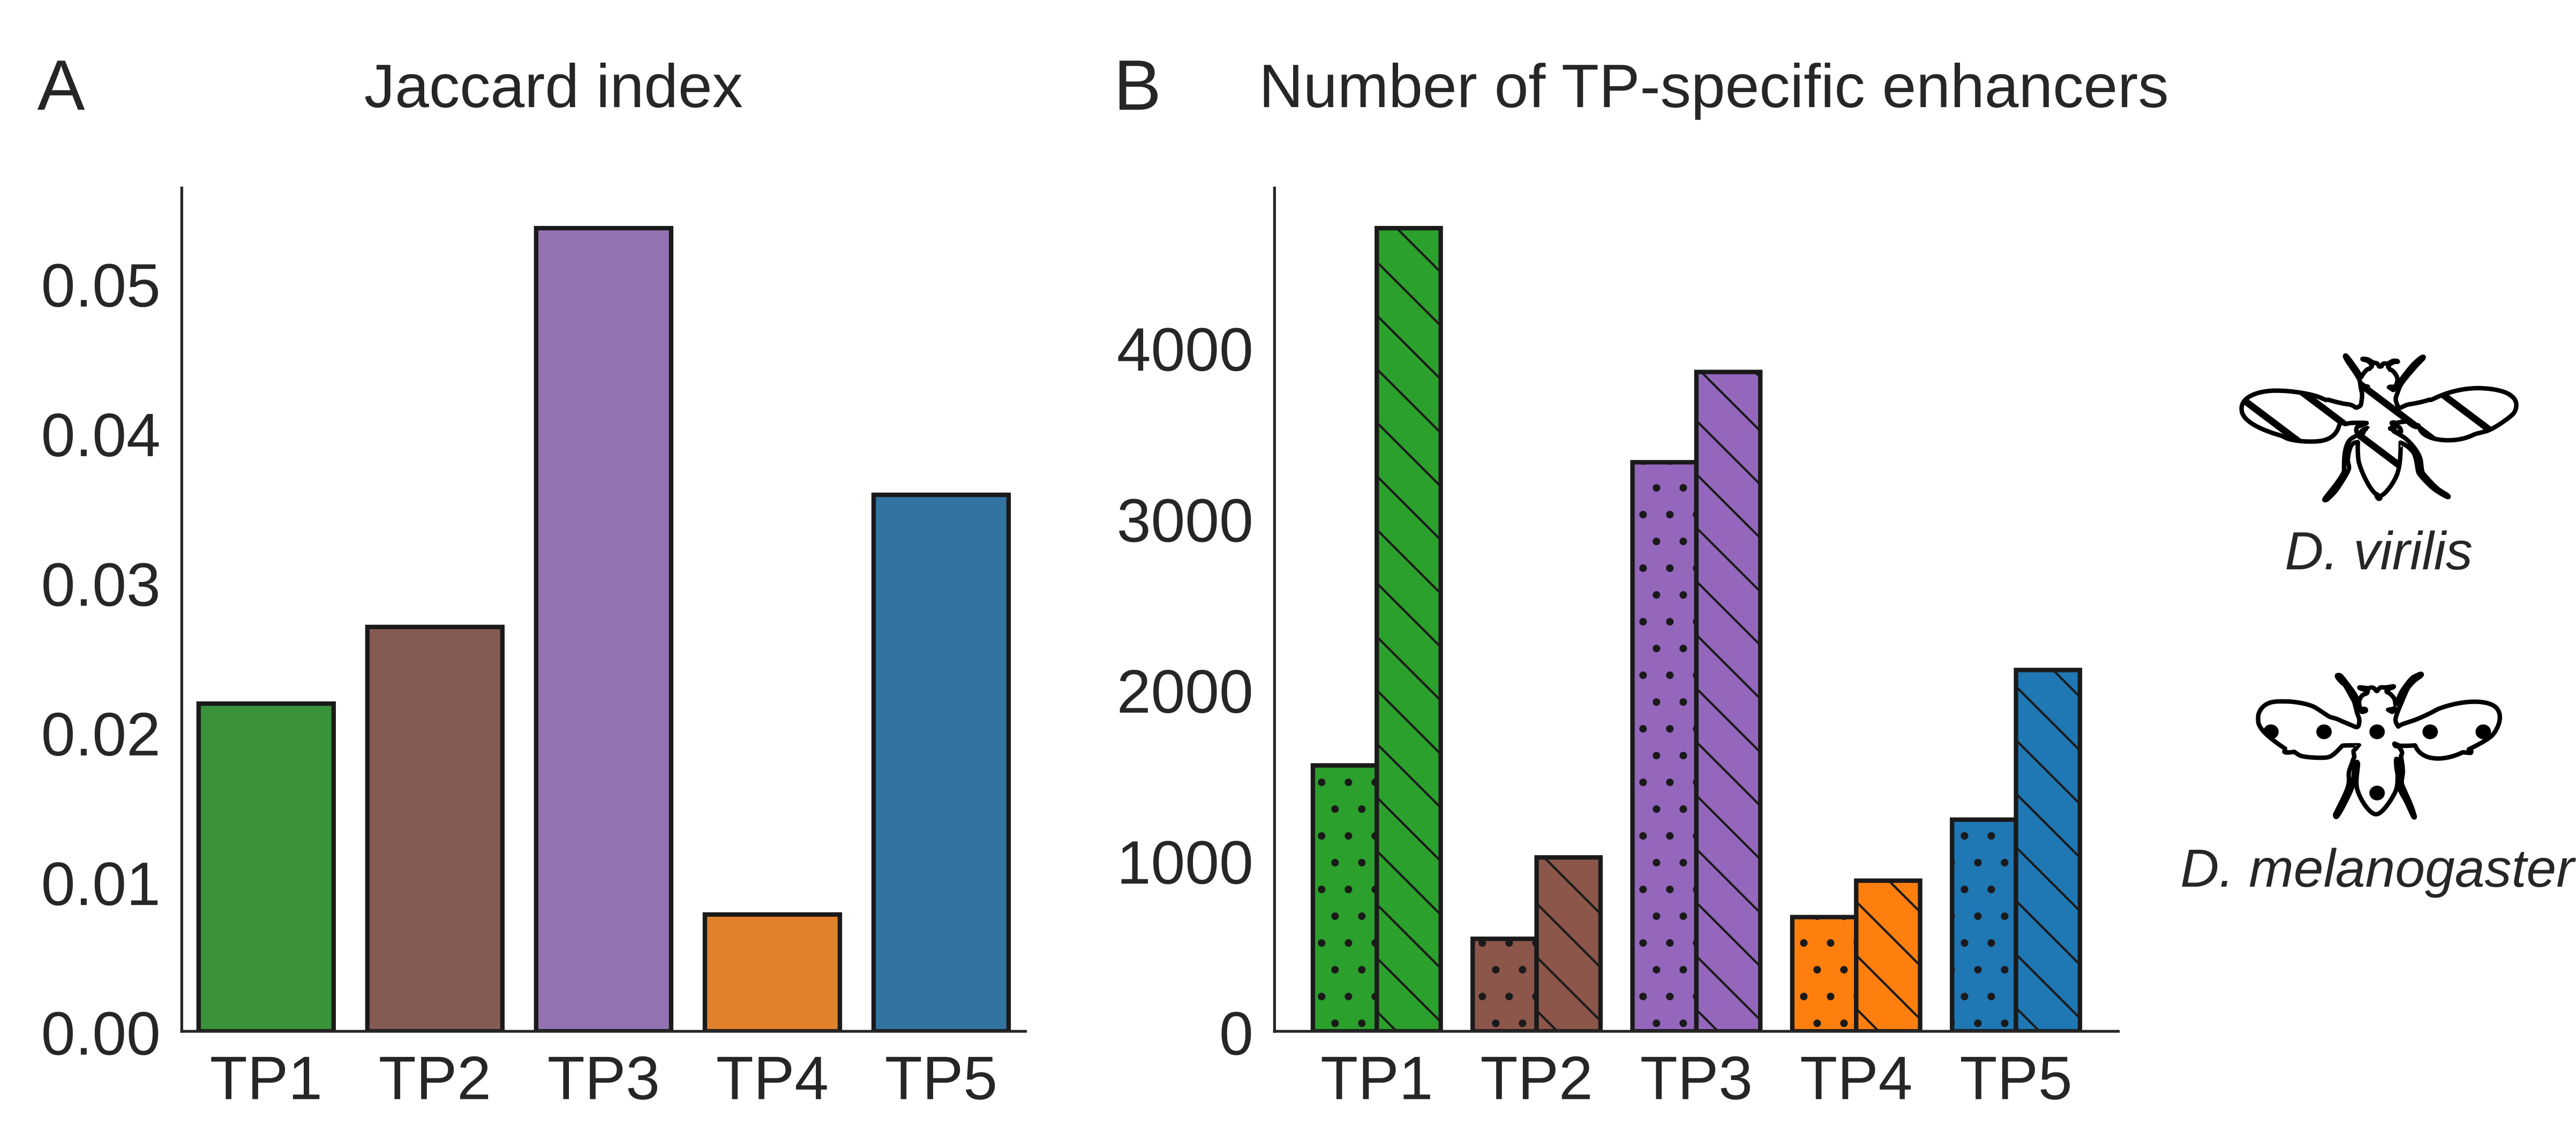
\includegraphics[width=\linewidth]{ch.hourglass/images/enhancers_between.png}
    \caption{\textbf{Temporal similarity between \textit{D. virilis} and \textit{D. melanogaster}.} \textbf{(A)} The proportion of conserved stage-specific enhancers at each development stage between \textit{D. melanogaster} and \textit{D. virilis}. TP1 corresponds to 2-3 HAEL (hours after egg laying), TP2: 6-8 HAEL, TP3: 10-12 HAEL, TP4: 14-16 HAEL, TP5: 18-20 HAEL. \textbf{(B)} The number of time point specific enhacers for \textit{D. melanogaster} and \textit{D. virilis} over time. }
    \label{fig:peak_between}
\end{figure}

To test whether a relationship between the number of TP-specific enhancers and the Jaccard index exists, we made a consensus set of enhancers for \textit{D. melanogaster} and \textit{D. virilis} over all time points. Each time point gets assigned a set of randomly picked enhancers, whilst keeping the original number of enhancers per time point. This removes all biological meaning from the data, thus if the analysis is unbiased it should generate equal Jaccard indexes for all time points. Yet TP3 clearly shows an enriched Jaccard index (Fig. \ref{fig:shuffle}A). This indicates that the number of enhancers per time point influences the analysis. The obvious way to control for this would be to subsample all time points to the same number of enhancers (Fig. \ref{fig:shuffle}B). After subsampling, we find that TP2 (6-8 hours after egg laying), a period that precedes the \textit{Drosophila} phylotypic stage\cite{Kalinka2010,Liu2020}, shows the highest conservation between enhancers between \textit{D. melanogaster} and \textit{D. virilis}. The dependence of the Jaccard index is also present in a within-species comparison between \textit{D. virilis} replicates. The dependence of the Jaccard index on the number of enhancers can also be formally established, see section \ref{subsection:flypeaks}.

\begin{figure}
    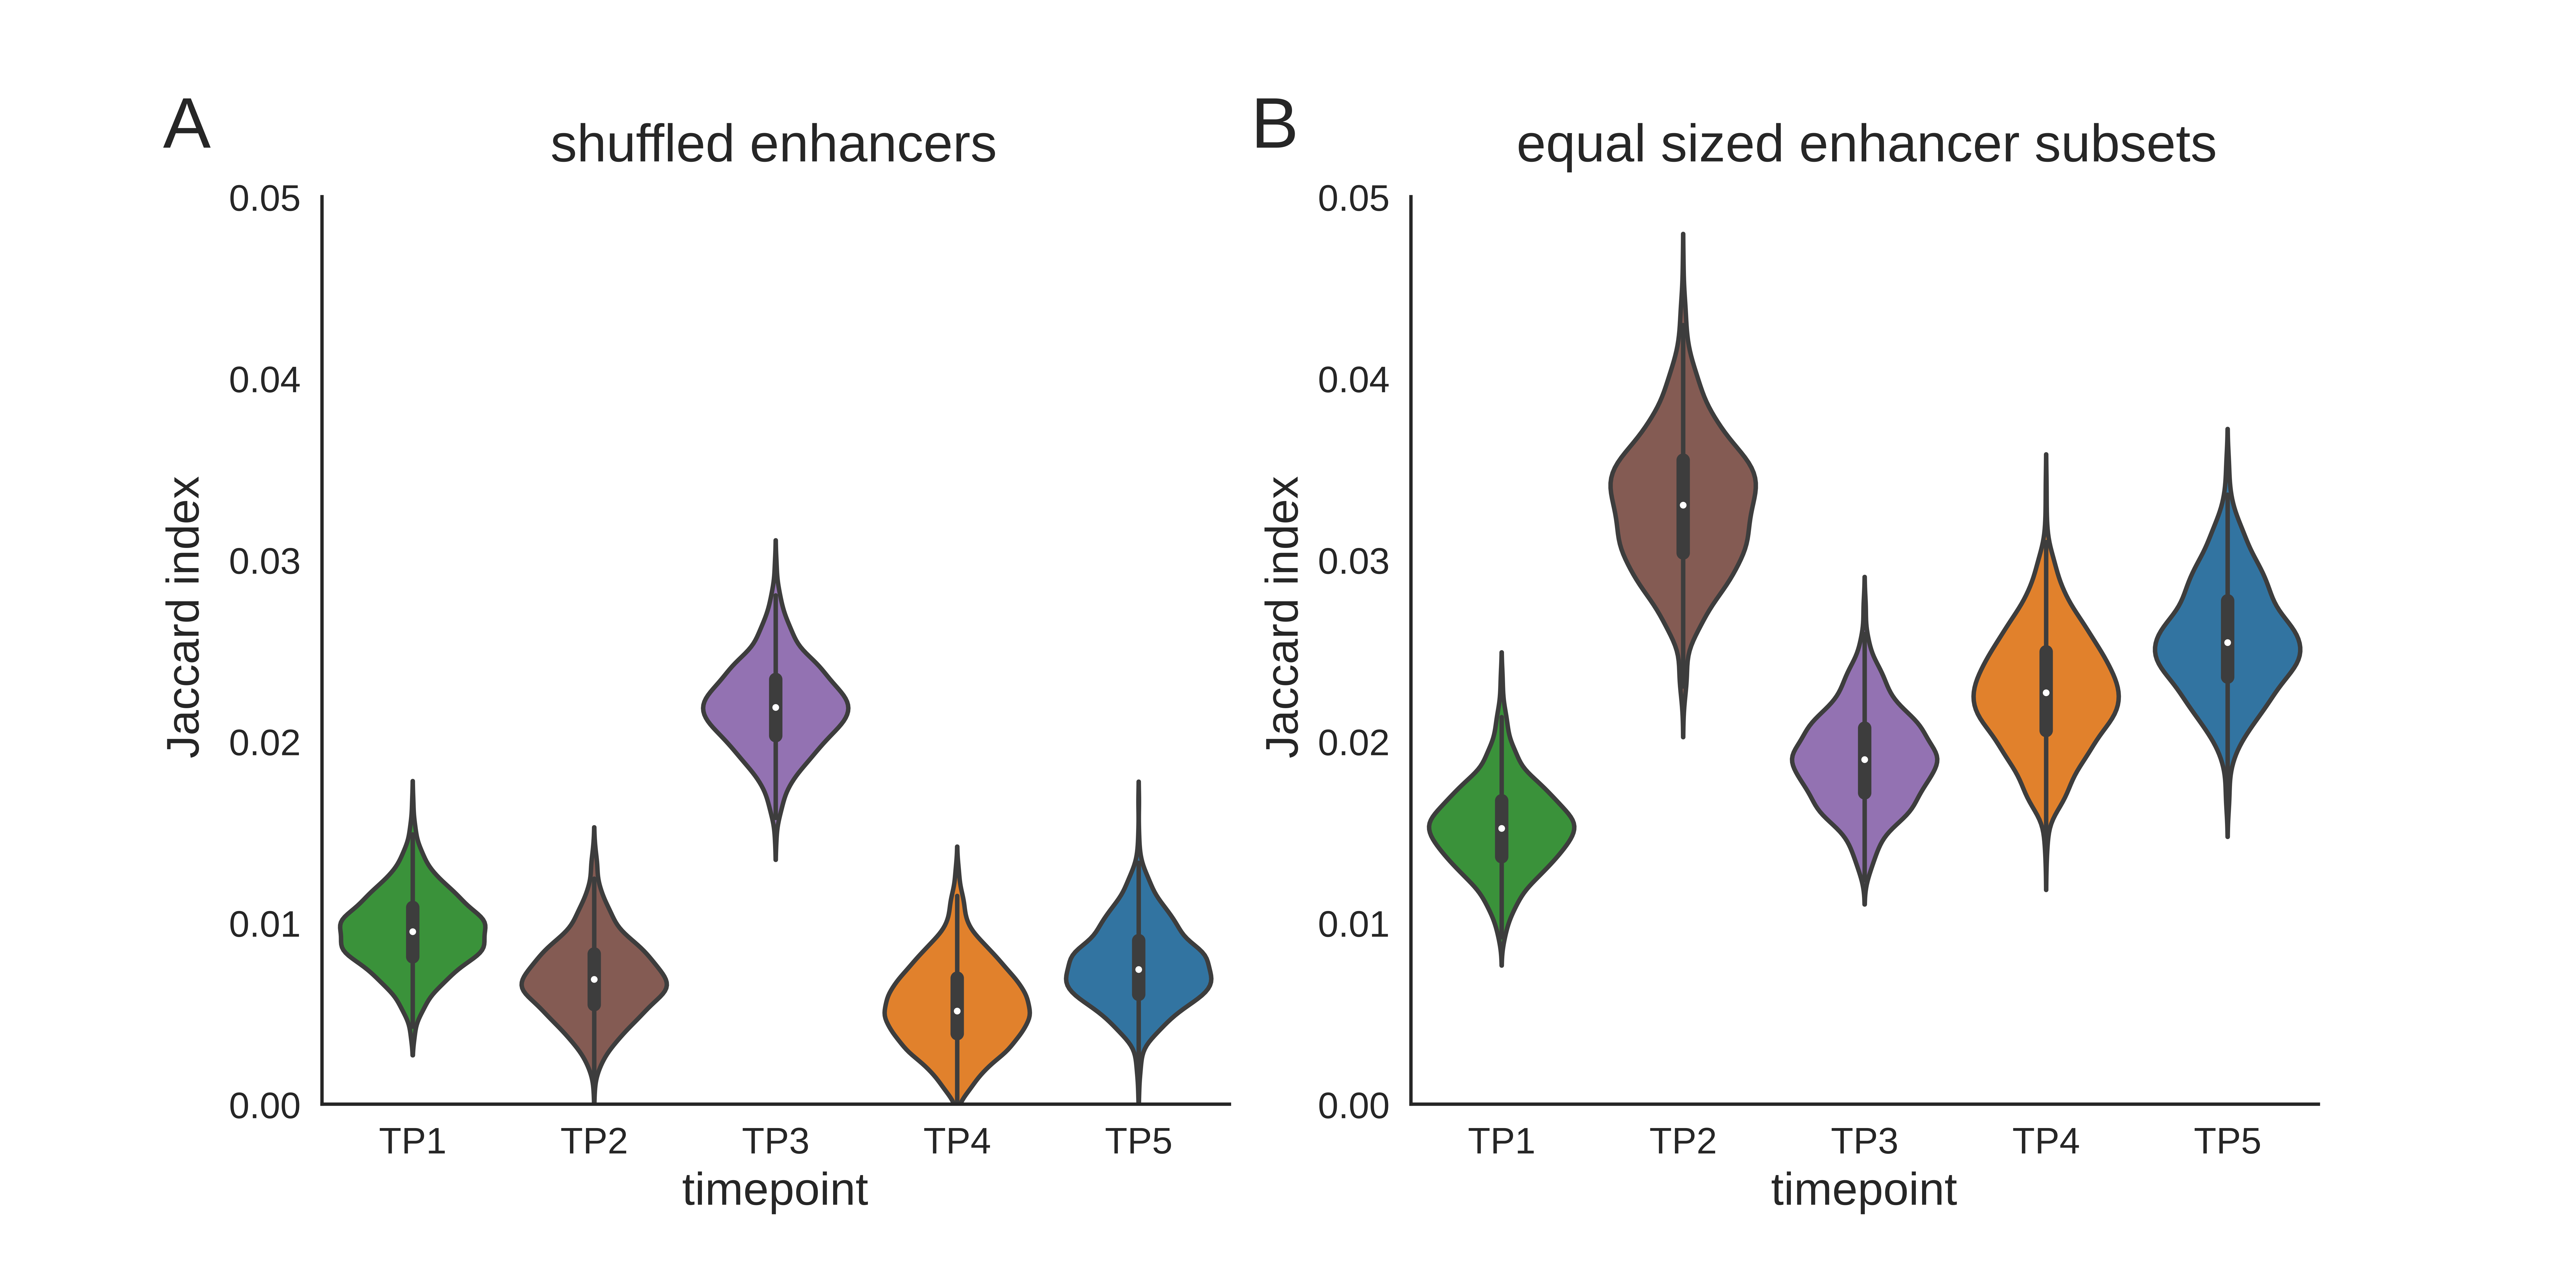
\includegraphics[width=0.9\linewidth]{ch.hourglass/images/fly_shuffle.png}
    \caption{\textbf{The Jaccard index depends on the number of enhancers.} \textbf{(A)} Distribution of Jaccard scores after randomly distributing enhancers to time points, but with an identical number of enhancers per time point as originally found (1,000 permutations). If the number of enhancers per time point does not influence the result an equal distribution is expected. The enrichment of TP3, however, indicates that this methodology is sensitive to the number of enhancers per time point ((\textit{dmel}, \textit{dvir}) TP1: (6,768, 12,150) TP2: (6,093, 8,334) TP3: (12,052, 13,404) TP4: (5,597, 5,941) TP5: (6,352, 8,390)). \textbf{(B)} Subsampling to 2,000 enhancers per time point (1,000 permutations). This removes the dependency of the Jaccard index on the number of enhancers. TP3 is not enriched after subsampling.}
    \label{fig:shuffle}
\end{figure}

Apart from a biological interpretation for the different number of TP-specific enhancers, there are also two methodological interpretations. First, the focus on TP-specific enhancers creates artificially separated sets of enhancers. TP-specific enhancers, as defined by Liu \textit{et al.}, are enhancers occurring at one time point only. This means that if two time points are sampled more closely in (developmental) time, these two time points would share most of their enhancers, resulting in a low number of TP-specific enhancers. This is something the authors themselves already note. Similarly, enhancers at the beginning and the end of the time series have a higher chance of being TP-specific purely because there is only one adjacent time point, whilst the rest of the time series are compared against two. A similar approach that doesn't suffer from the artificial separation, would be to visualize the percentage of reads in the consensus peak set in enhancers vs promoters per time point. Applied to this data we find no clear enrichment for enhancers for a specific time-point (Fig. \ref{fig:peak_enrichment}). Secondly, arbitrary thresholds are used during peak calling to decide whether a region is \textit{enriched}. This threshold depends, for instance, on the signal-to-noise ratio, which is expected to change for developing embryos, and the sequencing depth\cite{encode_guidelines2012}. Neither of these confounders has been corrected for in the original analysis.

Moreover, Liu \textit{et al.} proceed to train a computational model on the sequences of TP-specific enhancers of \textit{Drosophila}. This model is then used to determine per enhancer whether it has been subjective to positive or non-positive selection. They then find that the ratio of enhancers subjected to positive selection vs enhancers subjected to non-positive selection is high for TP1, TP3, and TP5, and thus conclude that the molecular basis for the phylotypic stage can partially be explained by positive selection of gene regulation conservation. Alternatively, there are two other likely (methodological) explanations for this pattern that have not been tested. The first explanation is, again, that as there has been no correction for signal-to-noise ratio and sequencing depth, there is a difference in the type(s) of peaks the pre-processing picked up, which in turn translates to different predicted positive selection ratios\cite{encode_guidelines2012,Whalen2021}. The second explanation is that, as is true for practically all machine learning, the model generalizes and performs better with more training data. Looking at their reported model performance (Fig. 3\cite{Liu2021}) we can see that the model's performance for TP1, TP3, and TP5 is notably higher than for TP2 and TP4. In figure \ref{fig:peak_within}B we see that the high model performance closely follows the amount of training data (number of TP-specific peaks). Simply speaking, a model that has been trained with more data generalizes better and appears to predict a higher amount of positive selection. Without a proper test for these potential confounders, it is hard to reach a definitive conclusion about positive selection concerning the hourglass model and the phylotypic stage.

In summary, in our re-analysis we reproduce the result that TP3 has the highest overlap between enhancers between \textit{D. melanogaster} and \textit{D. virilis}. However, the Jaccard index is dependent on the combination of biological similarity and the number of enhancers per time point. This dependence is visible when comparing \textit{D. virilis} replicates among themselves and when shuffling the data. Moreover, it is likely that the number of TP-specific enhancers also influences the downstream training of the gkm-SVM and in turn the pattern of enhancer positive selection. 

\section{Discussion}

Our study highlights the importance of including within-species, within-phylum, and between-phylum comparisons in the quantitative analysis of the phylotypic stage. We demonstrate that the high transcriptome similarity between \textit{D. rerio} and \textit{X. tropicalis} at the phylotypic stage\cite{marletaz2018} can be explained by within-species effects alone. Similarly, we show that the cell type proportion \say{hourglass-like} bottleneck between \textit{M. musculus} and \textit{O. cuniculus}\cite{Mayshar2023} is also caused by within-species effects. Furthermore, we identify the mid-developmental transition\cite{Levin2016} and \textit{Drosophila} enhancer conservation at the phylotypic stage\cite{Liu2021} as methodological artifacts. 

When comparing time series directly, it is important to control for statistical biases in the data, such as the correspondence between replicates, but also the temporal sampling strategy, data distribution, and gene sets used. A key bias that is often overlooked is whether the sampling schema follows developmental time\cite{BinindaEmonds2002}. It is not uncommon for studies to report a discontinuous blocked pattern of within-species correlation, where the difference between stages is not equal. This difference usually gets assigned a biological explanation; for instance as embryonic genome activation\cite{Yanai2011} or developmental milestones\cite{Levin2012}. However, this blocked within-species pattern proceeds to affect any downstream between-species comparison, where in turn the same blocks are visible. The only way to make a fair comparison between-species, however, is when the within-species similarity between all adjacent time points is equal (which corresponds to the null model within a time series of Fig. \ref{fig:models}), or if one explicitly corrects this bias statistically. When sampling stages closely in time, one increases the probability of stages matching closely in a comparison with another time series. This in turn increases the expected similarity. The reverse is also true, where stages sampled in large intervals reduce the probability of matching stages between time series, which then reduces the expected similarity. Under the assumption that embryonic development has no point of higher selective pressure, a comparison between two time series will have the highest expected similarity at the point where sampling has happened at the shortest interval. For this reason, we argue for a re-definition of molecular embryonic time, where not morphological features or absolute time post-fertilization is used, but where the (molecular) difference between adjacent stages is equal. 

A different potential bias is the changing gene expression distributions, which are a consequence of developmental maturity. It has been demonstrated that transcriptional entropy, a measure of disorder in a system, is decreasing over development\cite{Kannan2021}. Pluripotent tissues have relatively many genes activated, whilst more differentiated cells in mature tissues make use of a smaller, more specialized set of genes. These changing gene expression distributions during development can introduce unexpected biases and artifacts when calculating similarity. For instance, the JSD and Pearson correlation coefficient between two count tables from different distributions can never be maximal (respectively zero and one). As an effect, directly comparing similarity scores between time points can be misleading as the range of possible similarity scores is different per comparison. To circumvent this problem one can resort to non-parametric distance metrics, such as the rank-based Spearman correlation coefficient\cite{Irie2011}, or quantile normalizing the data before calculating the distance metric\cite{marletaz2018}. Then, one can compare the similarity scores directly, but these approaches ignore the biologically relevant gene expression distribution changes. As long as there is no consensus on what type of molecular similarity is expected at the phylotypic stage, it can both be correct as well as incorrect to ignore the distributional changes. 

Another point to consider is the changing proportions of cell types. An embryo is formed by all its cells together, and their combined signal is measured in the study of the molecular phylotypic stage. But not every cell type expresses the same number of transcripts\cite{Kim2023, Percharde2017}, which consequently gives cells with a high number of transcripts a higher importance in the (dis)similarity calculation. Moreover, molecular changes between embryos could be caused by changes in gene expression, but also by changes in cell type proportions, and most likely a combination of them. For example, during the vertebrate phylotypic stage the neural tissue is already highly developed and neural cells are relatively abundant. Could the high similarity at the vertebrate phylotypic stage be an effect of the over-representation of these neural cell types? Or, as another example, a practically universal feature of embryos is that they grow during development. But because of this growth, the surface (skin) to volume (organs) ratio changes, which in turn could explain the molecular phylotypic stage. We currently have no understanding of whether the molecular similarity at the phylotypic stage is based on cell type proportion similarity or whether it is based on gene expression similarity (or the combination of both). Only a single-cell approach can distinguish the effects of cell type proportion and gene expression, which is essential for better understanding the basis of the molecular phylotypic stage.

Finally, calculating a single similarity score between species seems like a gross oversimplification of the complexity of evolutionary development. When focusing on one-to-one orthologues features, all newly derived and lost features are ignored. For instance, we started our analysis with 21.154 genes for \textit{X. tropicalis} and 24,417 genes for \textit{D. rerio} respectively. However, if we focus only on one-to-one orthologs this gets reduced to 5,444 genes. This means that for this comparison specifically, we discard approximately three-quarters of our biological signal. To our knowledge, the only method that considers these relationships is the transcriptomic derivedness index\cite{Leong2021}. The transcriptome derivedness makes use of the average expression of orthogroups, where empty groups get assigned a gene expression of zero. But in turn this makes this approach vulnerable to Simpson's paradox, where the correspondence between lost and common genes is dominating the similarity instead of the similarity between common genes\cite{Saccenti2023}. Moreover, it is still vulnerable to changing levels of similarity between replicates over development, and requires a within-species control. Nevertheless, the transcriptomic derivedness index is currently the only approach to model all evolutionary relationships. Besides ortholog pairings, gene expression is regulated by the complex interplay of multiple gene regulatory mechanisms. For instance, a single differentially expressed transcription factor can affect thousands of downstream genes. Biological data is notoriously not independently and identically distributed. Whole-transcriptome comparisons are thus biased towards the largest groups of co-regulated genes. In addition, the fact that comparisons subsetted on different GO terms result in different conservational patterns is a clear indication that a single metric for whole-transcriptome similarity conceals the different layers of conservation at the phylotypic stage\cite{Malik2017,Gildor2019,Onimaru2021}.

In the past decades, there has been extensive research into the (molecular) basis of the phylotypic stage. Yet, as a field, we have neglected to explicitly define the various evolutionary-developmental models, their predictions, and their limitations. Currently, similarity is often defined on an arbitrary basis depending on the available data. However, due to differences in methodology, vastly different results are obtained  \cite{Piasecka2013,Dunn2018,Chan2021}. Furthermore, this unstructured approach leaves us unaware of nonconforming results as science tends to predominantly report positive findings, leaving us unaware of negative or inconclusive results. Regardless of the similarity metric used, does the hourglass model predict that maximal developmental similarity is a between-species effect? Or does it already exist when comparing replicates of the same species? There is an implicit expectation that a point of maximum similarity exists between species of the same phylum, and not between species of different phyla. Yet phyla are an artificial framework, and to date, no evolutionary process has been described that is exclusive along the 35 phyla stems\cite{hejnol2016}. In summary, the phylotypic stage lacks an explicit definition and there is conflicting evidence supporting its existence. The field must shift focus from generating more data and comparative analyses, and instead reflect on past observations while establishing a clear and falsifiable definition for the phylotypic stage. Without such a definition, our efforts remain unproductive.

\section{Material and Methods}

\subsection{Overview of public data}

Full sample tables can be obtained from \url{https://zenodo.org/doi/10.5281/zenodo.10457767}.

\subsubsection{Comparative analyses}

\textit{Xenopus tropicalis} transcriptomic time series data was obtained from DDBJ:PRJDB3785 \cite{Hu2017}, and NCBI:PRJNA275011 \cite{Owens2016}, and mapped against assembly UCB\_Xtro\_10.0. \textit{Danio rerio} transcriptomic time series data was obtained from NCBI:PRJNA416866 \cite{marletaz2018} and EBI-ENA:PRJEB7244 \cite{White2017} and mapped against assembly GRCz11. \textit{Drosophila melanogaster} transcriptomic time series data was obtained from NCBI:PRJNA527284 \cite{Liu2021} and mapped against assembly BDGP6.32. The \textit{Drosophila melanogaster} DNAse I data was obtained from EBI-ENA:PRJEB10089 \cite{Liu2020} and mapped against the dm6 assembly. The \textit{Drosophila virilis} DNAse I data was obtained from EBI-ENA:PRJEB10089 \cite{Liu2020} and mapped against the droVir3 assembly.

\subsubsection{Within-species temporal variance}

The within-species transcriptomic temporal variance is based on the data of EBI-ENA:PRJEB7244 \cite{White2017} (GRCz11), NCBI:PRJNA527284 \cite{Liu2021} (BDGP6.32), and NCBI:PRJNA345017 \cite{Zalts2017} (ce11).

\subsubsection{Per-embryo vs TPM normalisation}

Per-embryo vs TPM normalisation comparisons are based on the count tables directly provided by NCBI:PRJNA275011 \cite{Owens2016}.

\subsection{Transcriptome analyses}

Preprocessing of RNA-seq was done automatically by seq2science v0.9.8\cite{seq2science} using the rna-seq workflow. Public samples were downloaded from the Sequence Read Archive with the help of the NCBI e-utilities and pysradb\cite{Choudhary2019}. Genome assemblies UCB\_Xtro\_10.0 (\textit{X. tropicalis}), GRCz11 (\textit{D. rerio}), BDGP6.32 (\textit{D. melanogaster}), ce11 (\textit{C. elegans}) and GRCm38.p6 (\textit{M. musculus}) were downloaded with genomepy 0.13.0\cite{Frlich2023}. Reads were trimmed with fastp v0.20.1\cite{Chen2018} with default options. Reads were aligned with STAR v2.7.6a\cite{Dobin2012} with default options. Subsequently, duplicate reads were marked with Picard MarkDuplicates v2.23.8\cite{picard}. General alignment statistics were collected by samtools stats v1.14\cite{Danecek2021}. Read counting and summarizing to gene level was performed on filtered bam using HTSeq-count v0.12.4\cite{Anders2014}. TPM normalized gene counts were generated using genomepy based on longest transcript lengths. Quality control metrics were aggregated by MultiQC v1.14\cite{Ewels2016}. 

The within-species permutation test (Fig. \ref{fig:within_timepoint}) was performed by randomly choosing two replicates of the same time point and calculating their Spearman correlation coefficient, with 250 random pairs per time point.

Orthologs between species were derived by the gimmemotifs motif2factors command (v0.18.0). This command downloaded the genome assemblies of cattle (\textit{ARS-UCD1.2}), fruit fly (\textit{BDGP6.32}), lancetfish (\textit{BraLan2}), human (\textit{GRCh38.p13}), mouse (\textit{GRCm38.p6}), zebrafish (\textit{GRCz11}), frog (\textit{UCB\_Xtro\_10.0}), maize (\textit{Zm-B73-REFERENCE-NAM-5.0}), nematode (\textit{ce11}), chicken (\textit{galGal6}), tardigrade (\textit{nHd\_3.1}),	koala (\textit{phaCin\_unsw\_v4.1}), and turtle (\textit{rCheMyd1}) through genomepy\cite{Frlich2023}, and converted all transcripts to peptides with gffread 0.12.7\cite{Pertea2020}. Only the longest peptide per gene was kept, which was then provided to orthofinder 2.5.4\cite{Emms2019}.

For the re-analyses we then took the average TPM per time point, kept only the one-to-one orthologs per species-species comparison, and did similar processing as the original studies. Specifically for the re-analysis of Marl\'etaz \textit{et al.} we quantile normalized\cite{qnorm} the TPMs and calculated the Jensen-Shannon distance on a log2 scale with TPMs divided by a million. The \textit{absolute} JSD values are vastly different between our and the original analysis. This is because we opted to represent TPMs as probabilities (TPM divided by a million) and calculate JSD using a log base of 2. This causes the JSD to be bound between 0 and 1, which makes comparisons between different data sets easier as they are on the same scale. For the re-analysis of Levin \textit{et al.} we kept all genes with a minimum TPM of 10 or higher, and with at least a 2-fold change. Then we log10 transformed the remaining data and calculated the Pearson correlation coefficient.

\subsection{Enhancer conservation}

We had trouble closely reproducing the original results of Liu \textit{et al.}, so we have opted to use the original processed data for the between-species comparison, but our own processed data for the within-species comparisons as this data is missing. By closely reproducing the original results with their data it shows that our ortholog inference works similarly to theirs.

Preprocessing of the samples for the within-species comparisons was done automatically by seq2science v0.9.8\cite{seq2science} using the atac-seq workflow. Public samples were downloaded from the Sequence Read Archive with the help of the NCBI e-utilities and pysradb\cite{Choudhary2019}. Genome assemblies \textit{dm6} and \textit{droVir3} were downloaded with genomepy 0.13.0\cite{Frlich2023}. Paired-end reads were trimmed with fastp v0.20.1\cite{Chen2018} with default options. Reads were aligned with bwa-mem2 v2.2.1\cite{bwamem2} with options '-M'. Afterwards, duplicate reads were marked with Picard MarkDuplicates v2.23.8\cite{picard}. Before peak calling, paired-end info from reads was removed with seq2science so that both mates in a pair get used. The peak-calling effective genome size was estimated by khmer v2.0\cite{Crusoe2015} by calculating the number of unique k-mers with k being the average read length per sample. Peaks were called with macs2 v2.2.7\cite{Zhang2008} with options '--shift -100 --extsize 200 --nomodel --buffer-size 10000' in BAM mode. A consensus set of all summits was made with gimmemotifs 0.17.2\cite{Bruse_2018}. We then removed all summits that fall within a TSS with pyranges v0.0.120\cite{Stovner2019} to only keep enhancers.

For the between-species comparison, we used pslmap to map all \textit{droVir3} enhancers to the \textit{dm6} assembly and only kept one-to-one orthologous regions.  This is not necessary for the within-species comparisons. Time-point-specific enhancers are defined as enhancers of which the summits are more than 200 base pairs removed from the enhancers of other time points. Overlap over time is calculated as the Jaccard index.

Permutation tests were performed on a table where the rows are the enhancers and the columns time points, and where each value is whether or not for that enhancer-time point combination the enhancer is called as a peak. We then randomly shuffled each column separately, so that the total number of enhancers stays the same, but the biological structure is removed from the data. On these tables, we then calculated the Jaccard index, and we repeated the process 1,000 times to get a distribution. Similarly, for the subsetted data, we took a random subset of 2,000 rows (enhancers) and calculated the Jaccard index on this. We similarly repeated this 1,000 times to get a distribution.

\subsection{Cell proportion re-analysis}

The table containing the inferred cell type proportions, including the color per cell type, were shared with us directly over email. Pairwise Pearson correlation coefficients were calculated and the corresponding area graphs were added to each time series.

\subsection{Code availability}

The final analysis can be found at \url{https://github.com/vanheeringen-lab/phylotypic_hourglass}.

\section{Acknowledgments}

We would like to thank Jialin Liu for his quick response to queries about the \textit{Drosophila} transcriptome dataset, Eileen Furlong for her help with processing the DNAse \textit{Drosophila} samples, Michal Levin and Itai Yanai for sharing their original orthology dataset, Ofir Raz for sharing the mouse and rabbit data, David Emms for help with questions about orthofinder, Mike Keesey for developing Phylopic and finally Eivind Fonn for his help with formalizing the mathematical derivations.

\section{Supplementals}

\subsection{Mid-developmental transition derivation}\label{subsection:middevelopmenttransition}

A basic proof that the mid-developmental transition is a methodological artifact follows relatively easily from the thought experiment where a gene starts the time series in an \textit{off} state, and at random switches to an \textit{on} state somewhere along this time series:

\begin{align*}    
    G(t) & = \begin{cases} \text{off},& t < t_{\text{activate}} \\ \text{on},& t \geq t_{\text{activate}} \end{cases} \quad \textrm{and} \quad
    t_{\text{activate}} = \text{Uniform}(0, 1) \quad \textrm{and} \quad
    0 \leq t \leq 1
\end{align*}

then:

\begin{align*}
    P(G(t) & = \text{on}) = t \\
    P(G(t) & = \text{off}) = 1 - t
\end{align*}

If we now assume we have two of these time series (x and y), we can define the probabilities that both genes are in the same state for $t_x$ and $t_y$:

\begin{align*}
    P(G(t_x) = G(t_y)) & = P(G(t_x) = \text{on}) \cdot P(G(t_y) = \text{on}) + P(G(t_x) = \text{off}) \cdot P(G(t_y) = \text{off}) \\
    & = t_x \cdot t_y + (1 - t_x) \cdot (1-t_y)
\end{align*}

When visualizing the probability for equality over all x and y a mid-developmental transition becomes clear (fig. \ref{fig:inverse_math}).

\subsection{Jaccard index}\label{subsection:flypeaks}

We assume that all enhancers are conserved between species $x$ and $y$. Moreover, we assume that our pre-processing randomly finds enhancers for each time-point with chance $\alpha_{ts}$, where $t$ represents the time-point and $s$ represents the species. We can calculate the number of time-point specific peaks for $U_{ts}$ in this case as:

\begin{align*}
    E & \text{ is the collection of all conserved enhancers between species } x \text{ and } y \\
    U_{ts} & \text{ represents the time-point specific enhancers for species } s \text{ at time point } t \\
    |U_{ts}| & = \alpha_{ts} \beta_{ts} |E|, \text{ where } \beta_{ts} = \prod_{i \in \{1, 2, 3, 4, 5\}\setminus\{t\}} (1 - \alpha_{is}) \\
\end{align*}

Where $\beta_{ts}$ represents the fraction of enhancers that are still eligible to be time-point specific. We can now calculate the expected overlap (union) between two time points of species $x$ and $y$:

\begin{align*}
    \mathbb{E}(|U_{tx} \cap U_{ty}|) & = |U_{tx}| * \frac{|U_{ty}|}{|E|} \\
    & = \alpha_{tx} \beta_{tx} |E| * \frac{\alpha_{ty} \beta_{ty} |E|}{|E|} \\
    & = \alpha_{tx} \beta_{tx} \alpha_{ty} \beta_{ty} |E| \\
\end{align*}

From this we can calculate the expected Jaccard index:

\begin{align*}
    Jaccard(U_{tx}, U_{ty}) & = \frac{|U_{tx} \cap U_{ty}|}{|U_{tx} \cup U_{ty}|} \\
    & = \frac{|U_{tx} \cap U_{ty}|}{|U_{tx}| + |U_{ty}| - |U_{tx} \cap U_{ty}|} \\
    & = \frac{\alpha_{tx} \beta_{tx} \alpha_{ty} \beta_{ty} |E|}{(\alpha_{tx} \beta_{tx} + \alpha_{ty} \beta_{ty} - \alpha_{tx} \beta_{tx} \alpha_{ty} \beta_{ty})|E|} \\
    & = \frac{\alpha_{tx} \beta_{tx} \alpha_{ty} \beta_{ty}}{\alpha_{tx} \beta_{tx} + \alpha_{ty} \beta_{ty} - \alpha_{tx} \beta_{tx} \alpha_{ty} \beta_{ty}}
\end{align*}

For simplicity we assume that all found enhancers are time-point specific ($\beta_{ts} = 1$), simplifying the formula to:

\begin{align*}
    Jaccard(U_{tx}, U_{ty}) & = \frac{\alpha_{tx} \alpha_{ty}}{\alpha_{tx} + \alpha_{ty} - \alpha_{tx} \alpha_{ty}}
\end{align*}

We can now visualize the Jaccard index for different $\alpha_{ts}$ values and can see a clear dependence on the fraction of enhancers found and the Jaccard index (Fig. \ref{fig:peak_math}). From this, it is clear that we need to correct for the number of enhancers. $\beta_{ts}$ only influences the height of the Jaccard index, but not the pattern.

\subsection{Supplemental figures}
\beginsupplement

\begin{figure}[H]
    \center
    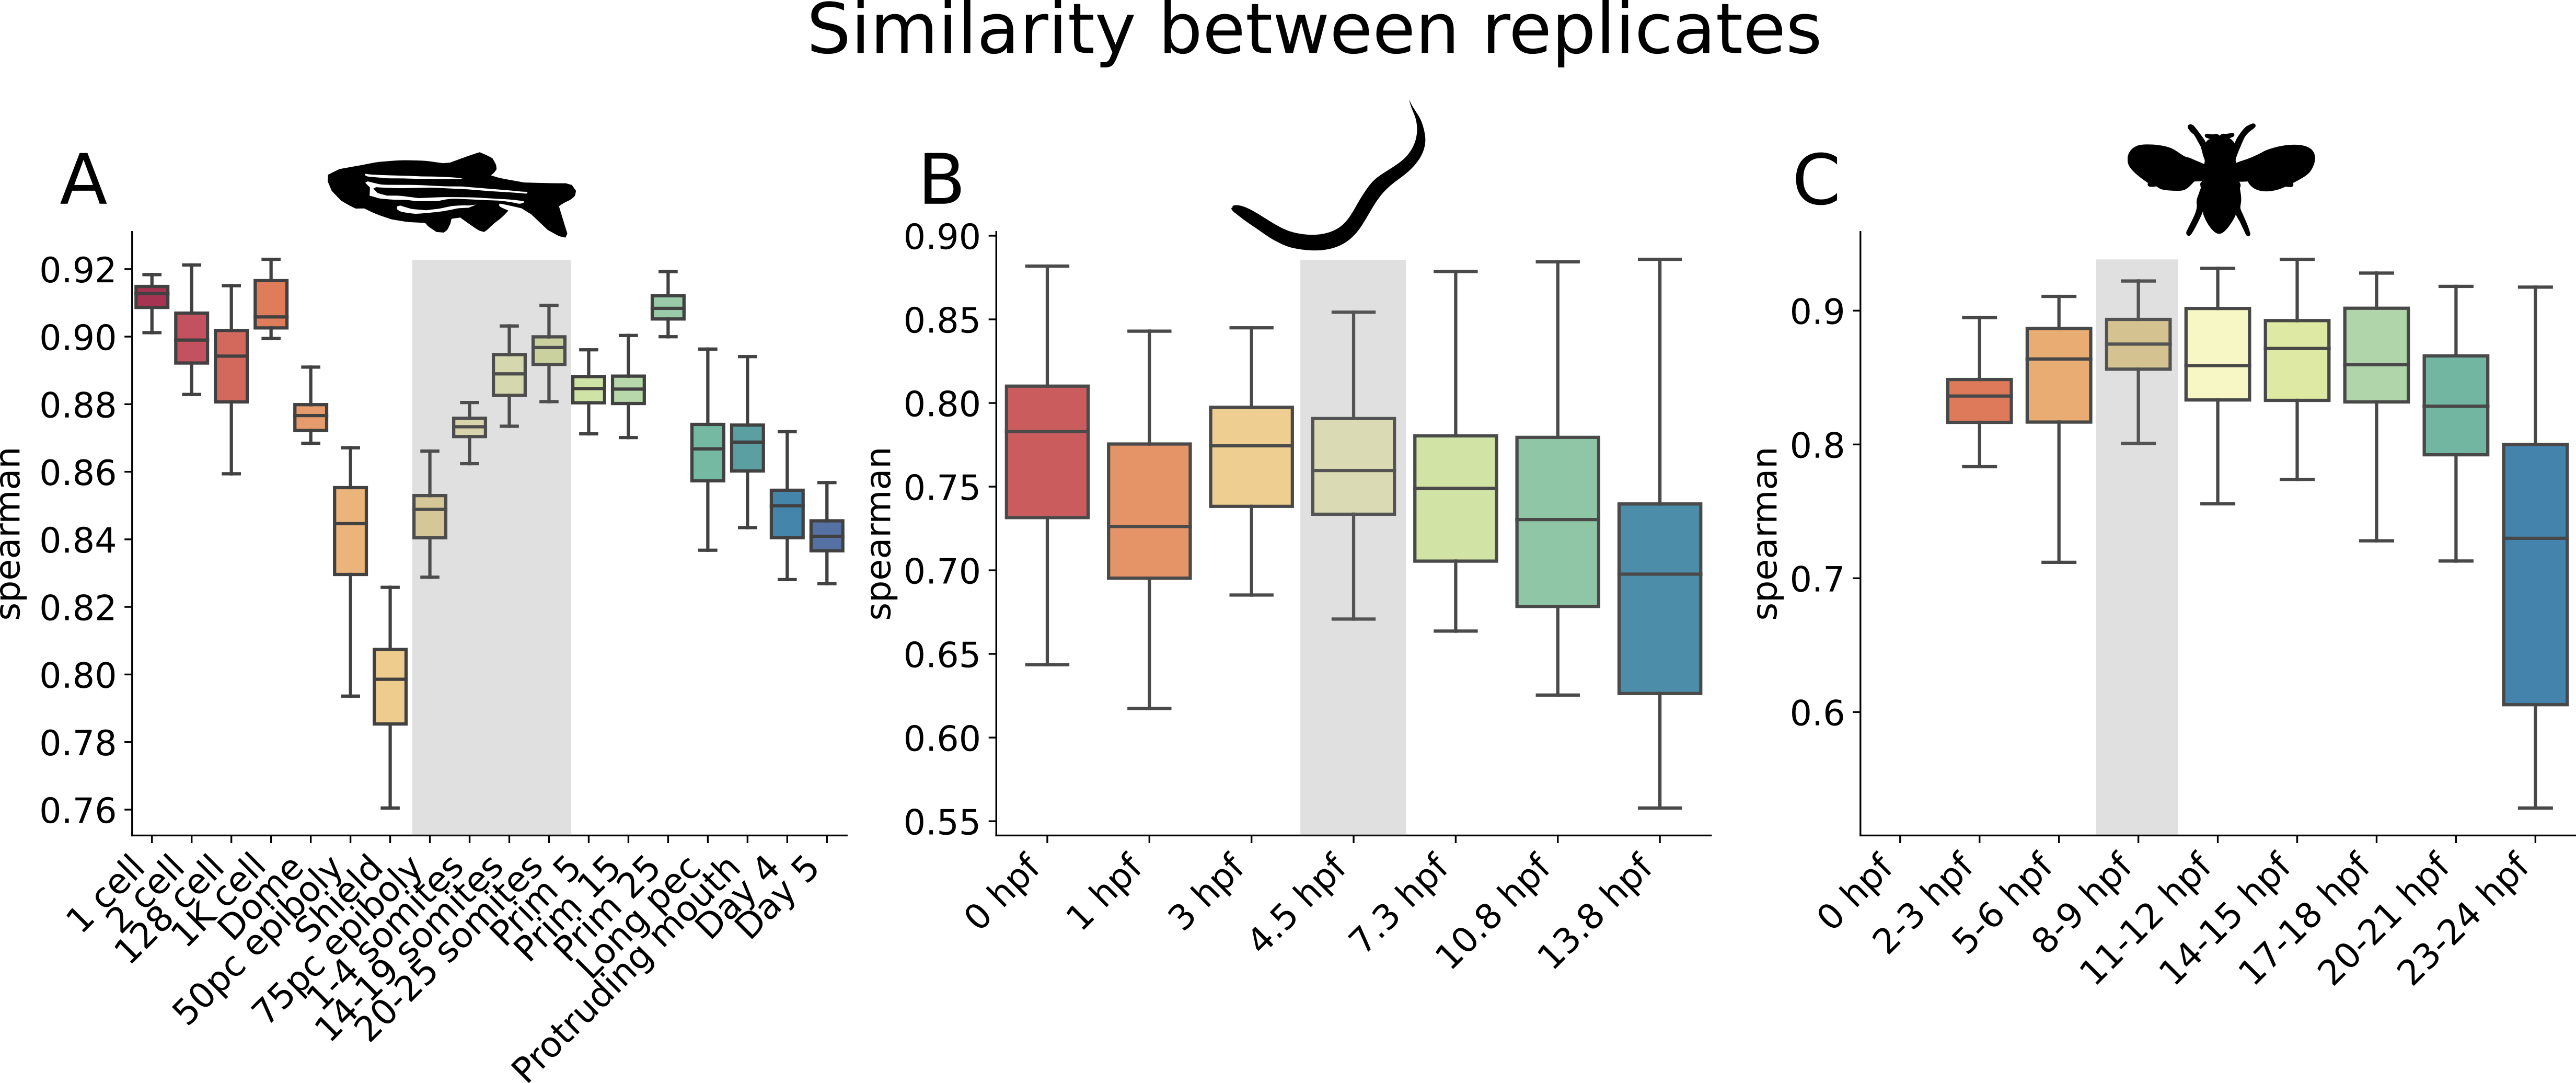
\includegraphics[width=\linewidth]{ch.hourglass/images/within_timepoint.png}
    \caption{\textbf{Changing levels of similarity between replicates is a potential cause for bias.} Boxplots of gene expression Spearman correlation coefficients between replicates belonging to the same stage for (A) single embryo \textit{D. rerio} samples, (B) pools of 10 \textit{C. elegans} embryos, and (C) single-embryo \textit{D. melanogaster} samples. The data is based on 250 randomly sampled pairs of replicates. The shaded area indicates the phylotypic stage. Note that all three species display a seemingly similar pattern, with high similarity between replicates at the start and mid-development. And a drop in early and late development. There are many potential causes for the changing levels of similarity over time; more biological variation between replicates at certain stages, a stage spanning too much time, or inversely a rapid development during certain stages, lab protocols that are optimized for certain stages and not others, etc.}
    \label{fig:within_timepoint}
\end{figure}

\begin{figure}[H]
    \center
    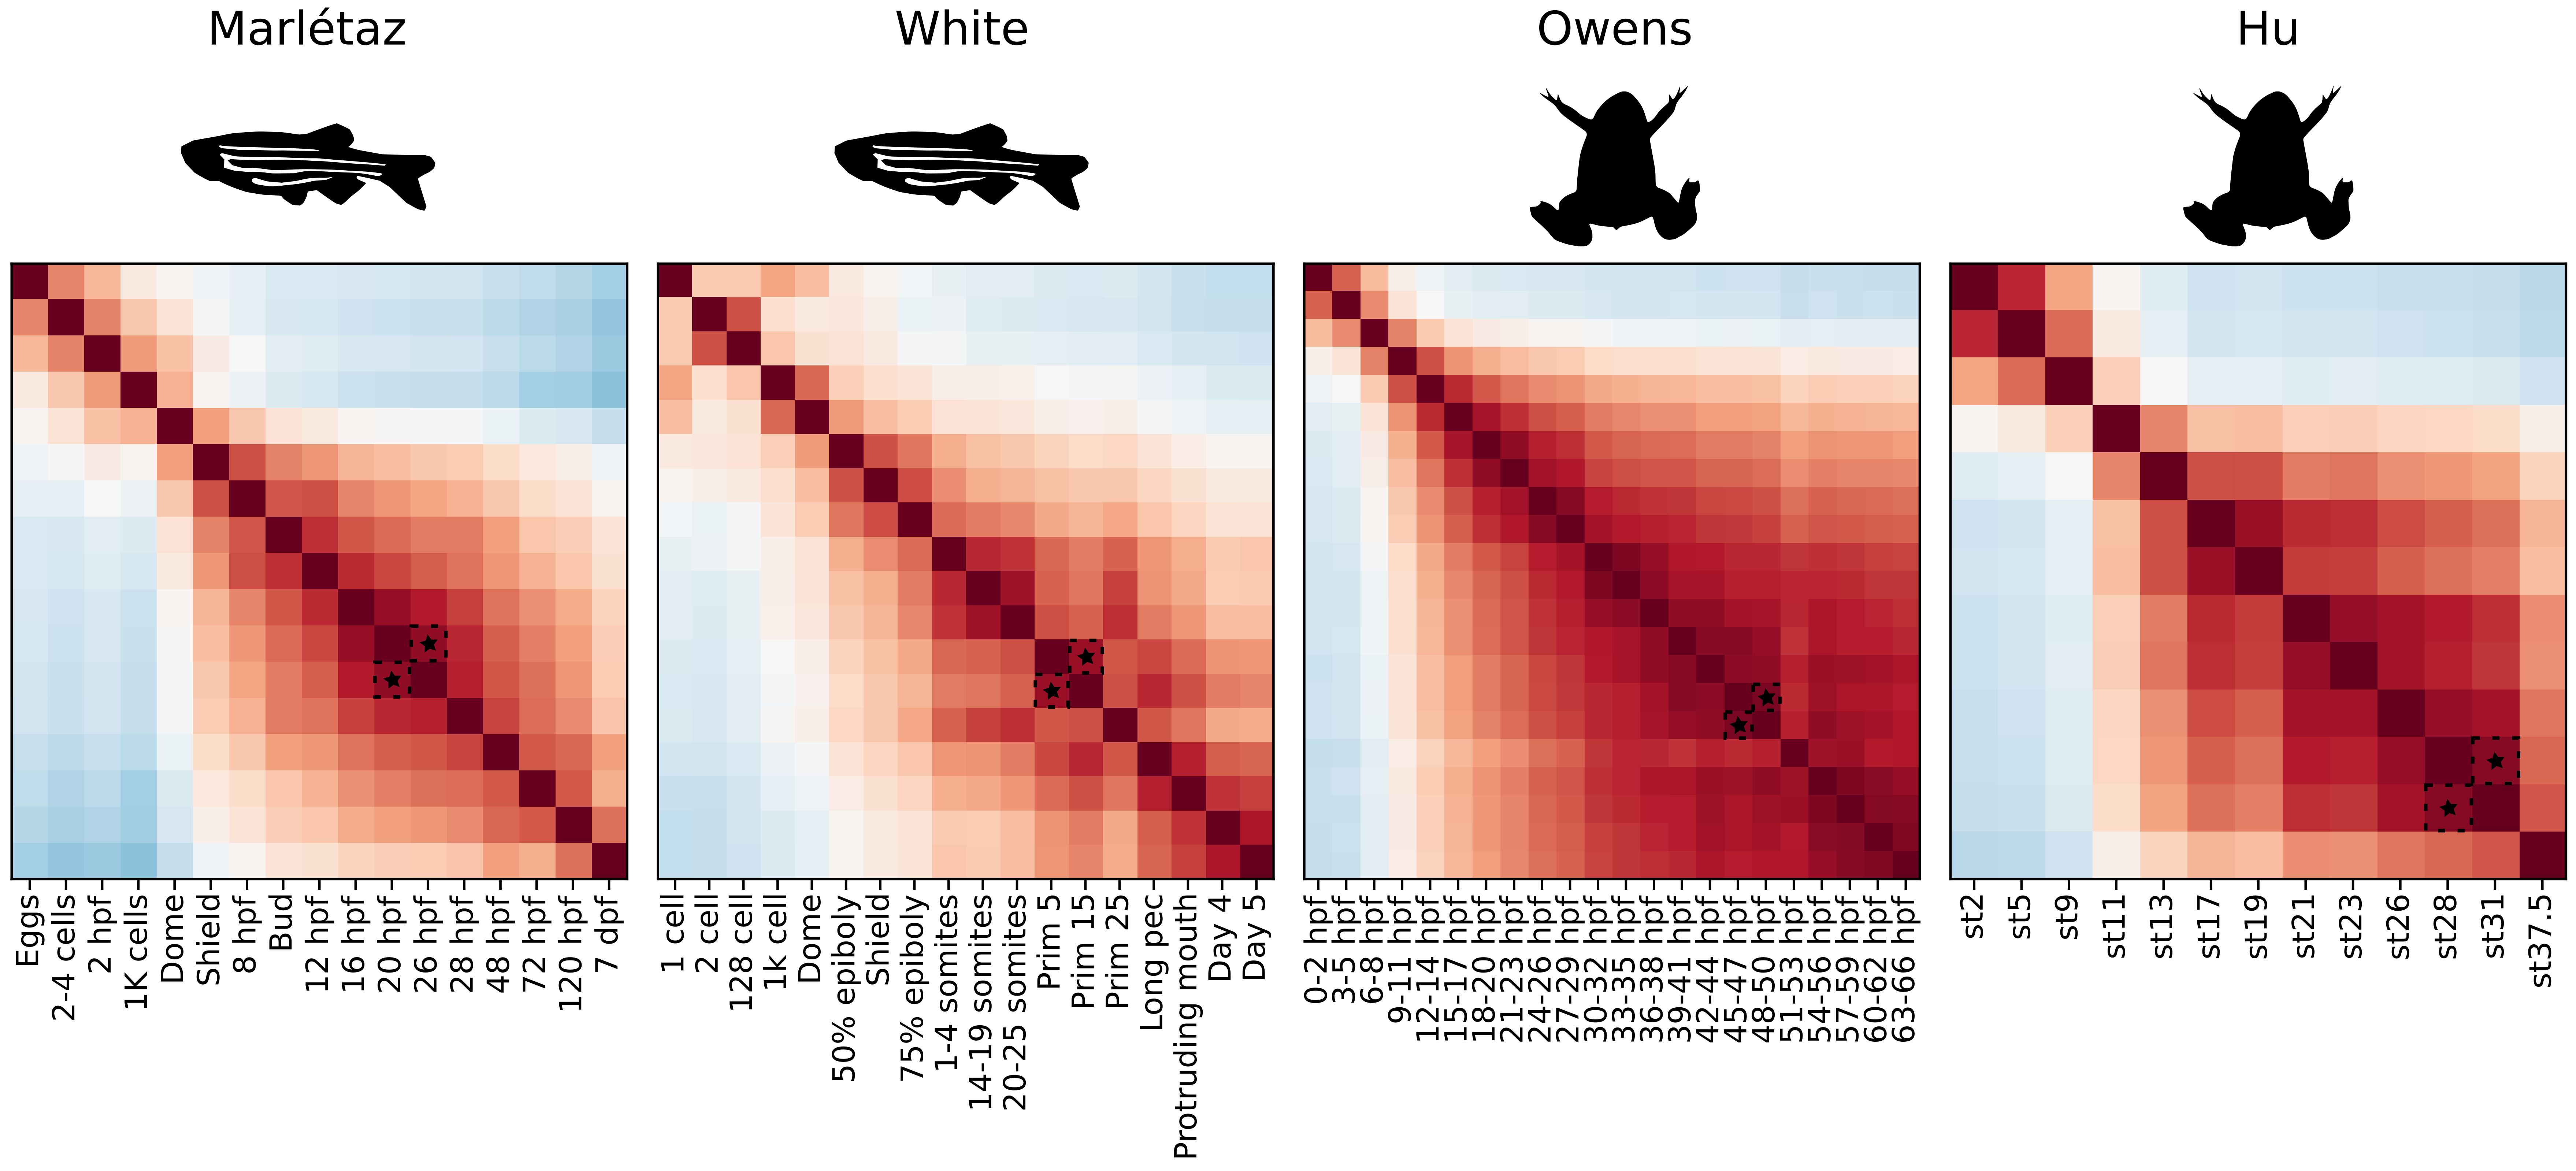
\includegraphics[width=\linewidth]{ch.hourglass/images/within_experiment.png}
    \caption{\textbf{High self-correlations at the phylotypic stage.} Heatmaps of pairwise Jensen Shannon Distances. Note how some series already display an hourglass-like pattern. Also note that the highest similarity between \textit{X. tropicalis} and \textit{D. rerio} in figure \ref{fig:betweenexperiment} corresponds to the highest self-similarity for \textit{D. rerio} (Marl\'etaz).}
    \label{fig:withinexperiment}
\end{figure}

\begin{figure}[H]
    \center
    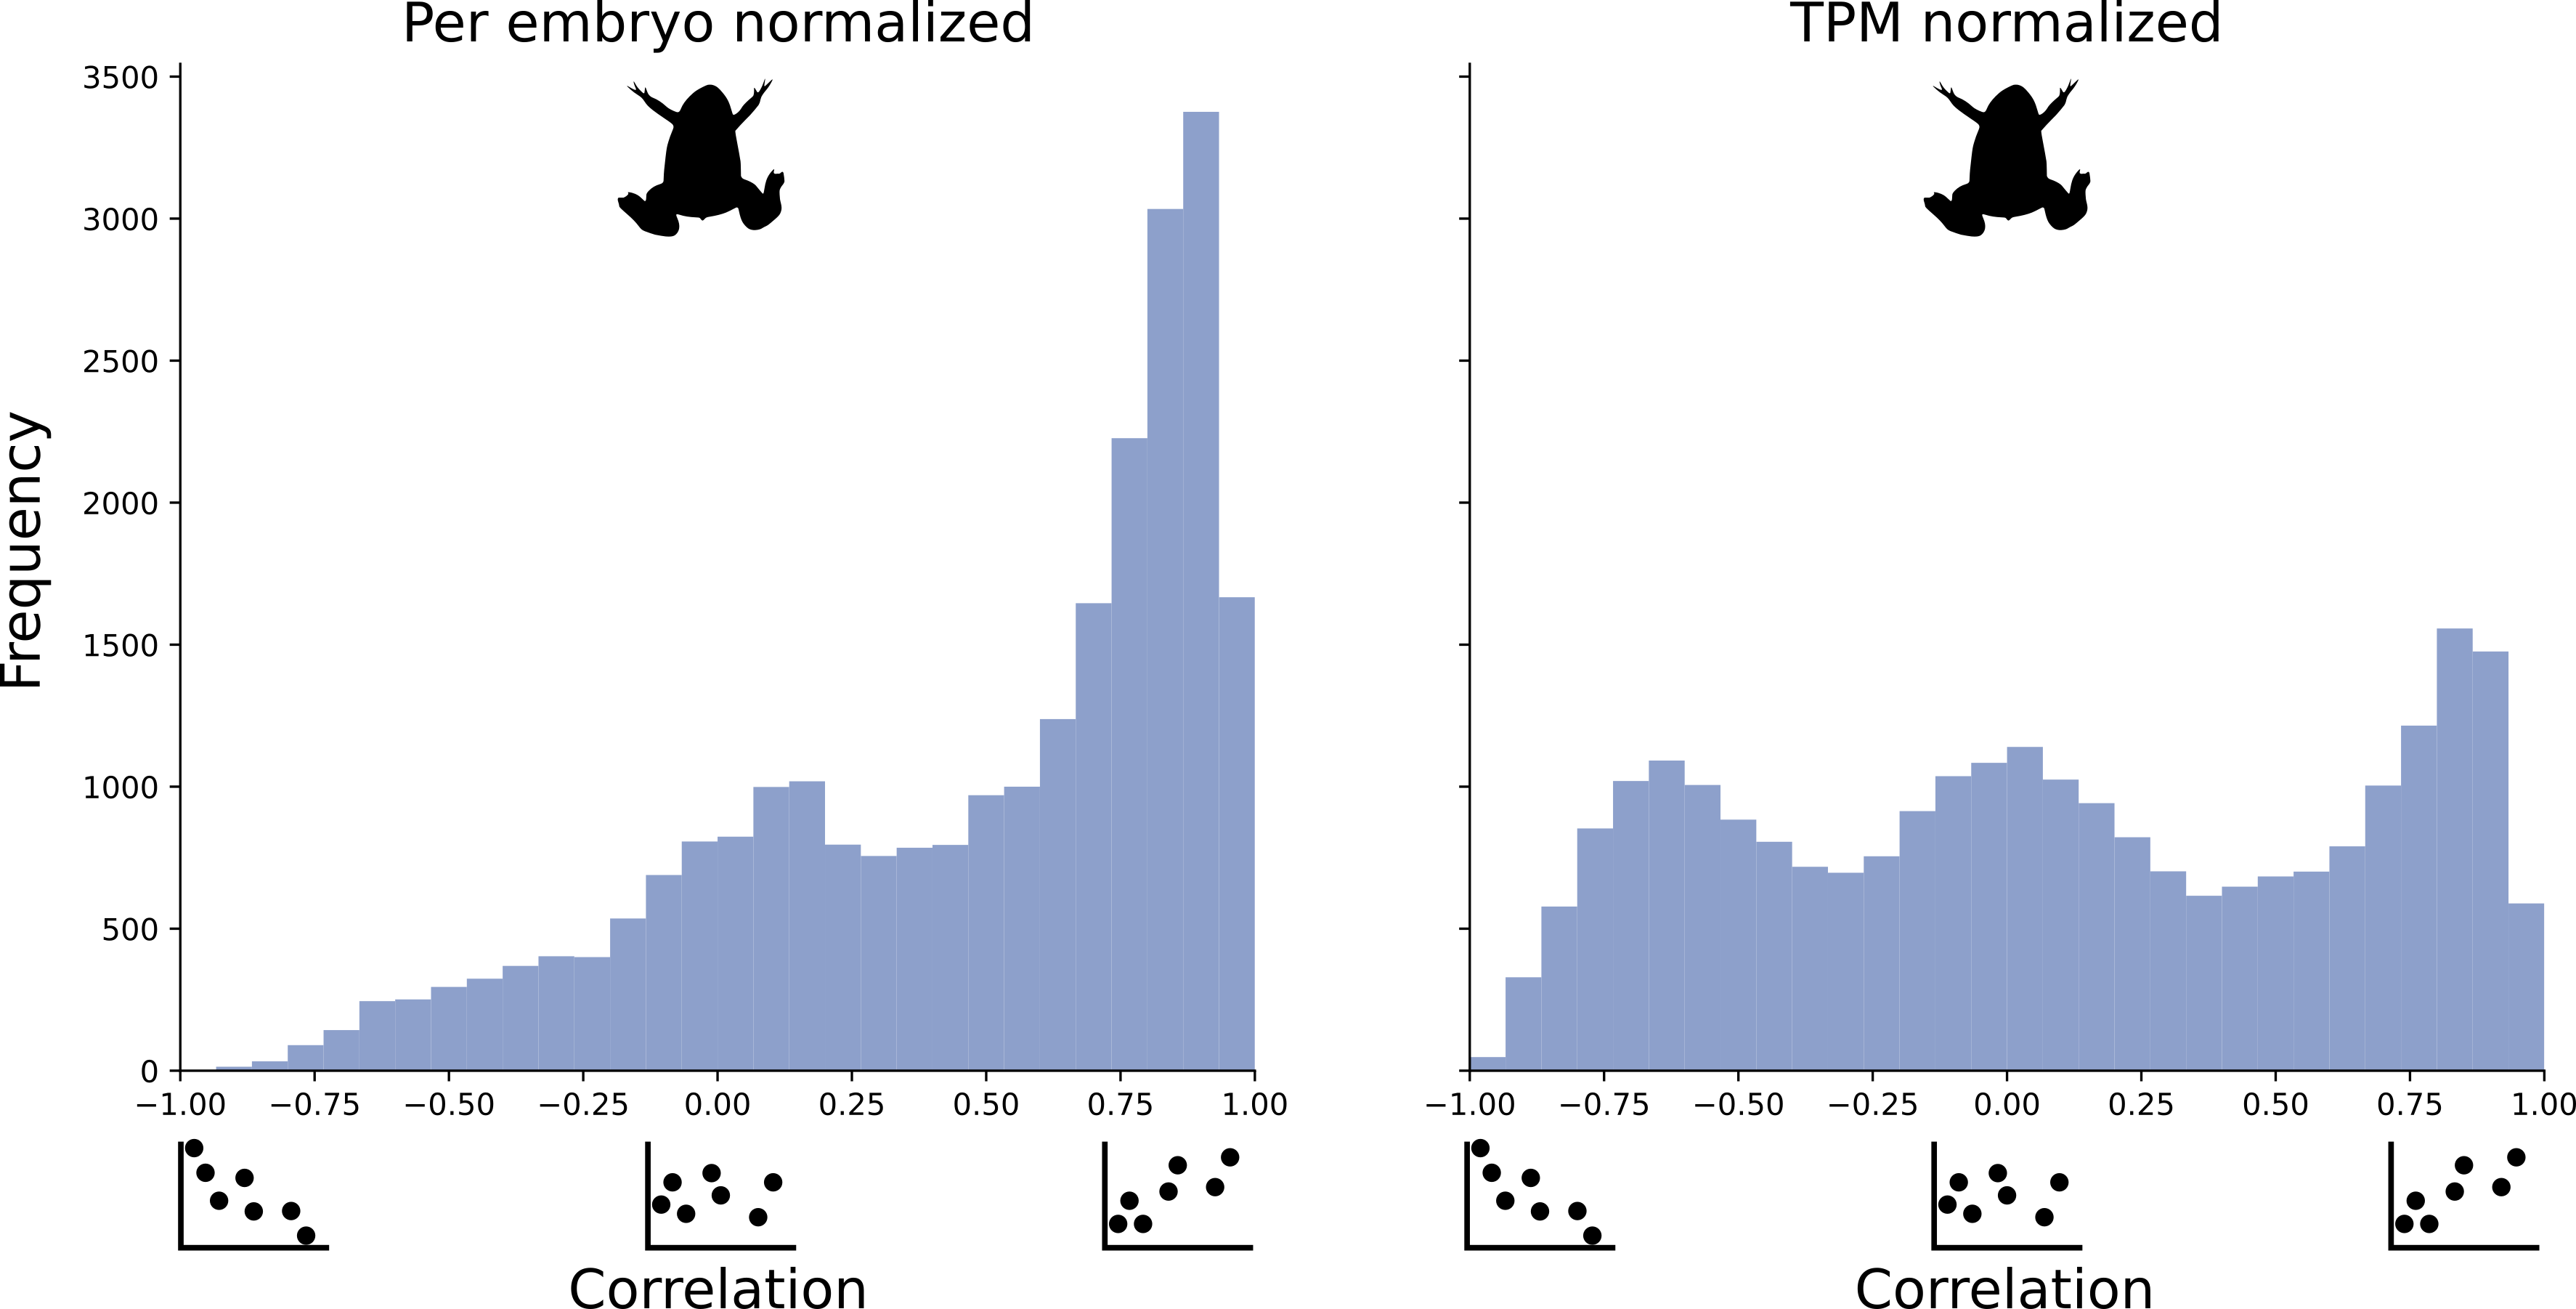
\includegraphics[width=0.75\linewidth]{ch.hourglass/images/gene_landscape_normalization.png}
    \caption{\textbf{The global per-embryo and TPM normalized gene expression patterns are vastly different for developing \textit{X. tropicalis} embryos.} Histograms of gene landscapes between per-embryo normalization and TPM normalization of \textit{X. tropicalis}. The left panel shows the gene landscape of per-embryo normalized gene expression. Because the \textit{X. tropicalis} embryo grows in size practically all genes are upregulated on a per-embryo level. In the right panel, the gene landscape of TPM normalized gene expression is visualized. Here we see that there are roughly three groups of gene expression, a down-regulated, a constant, and an up-regulated group.}
    \label{fig:genelandscapenormalization}
\end{figure}

\begin{figure}[H]
    \center
    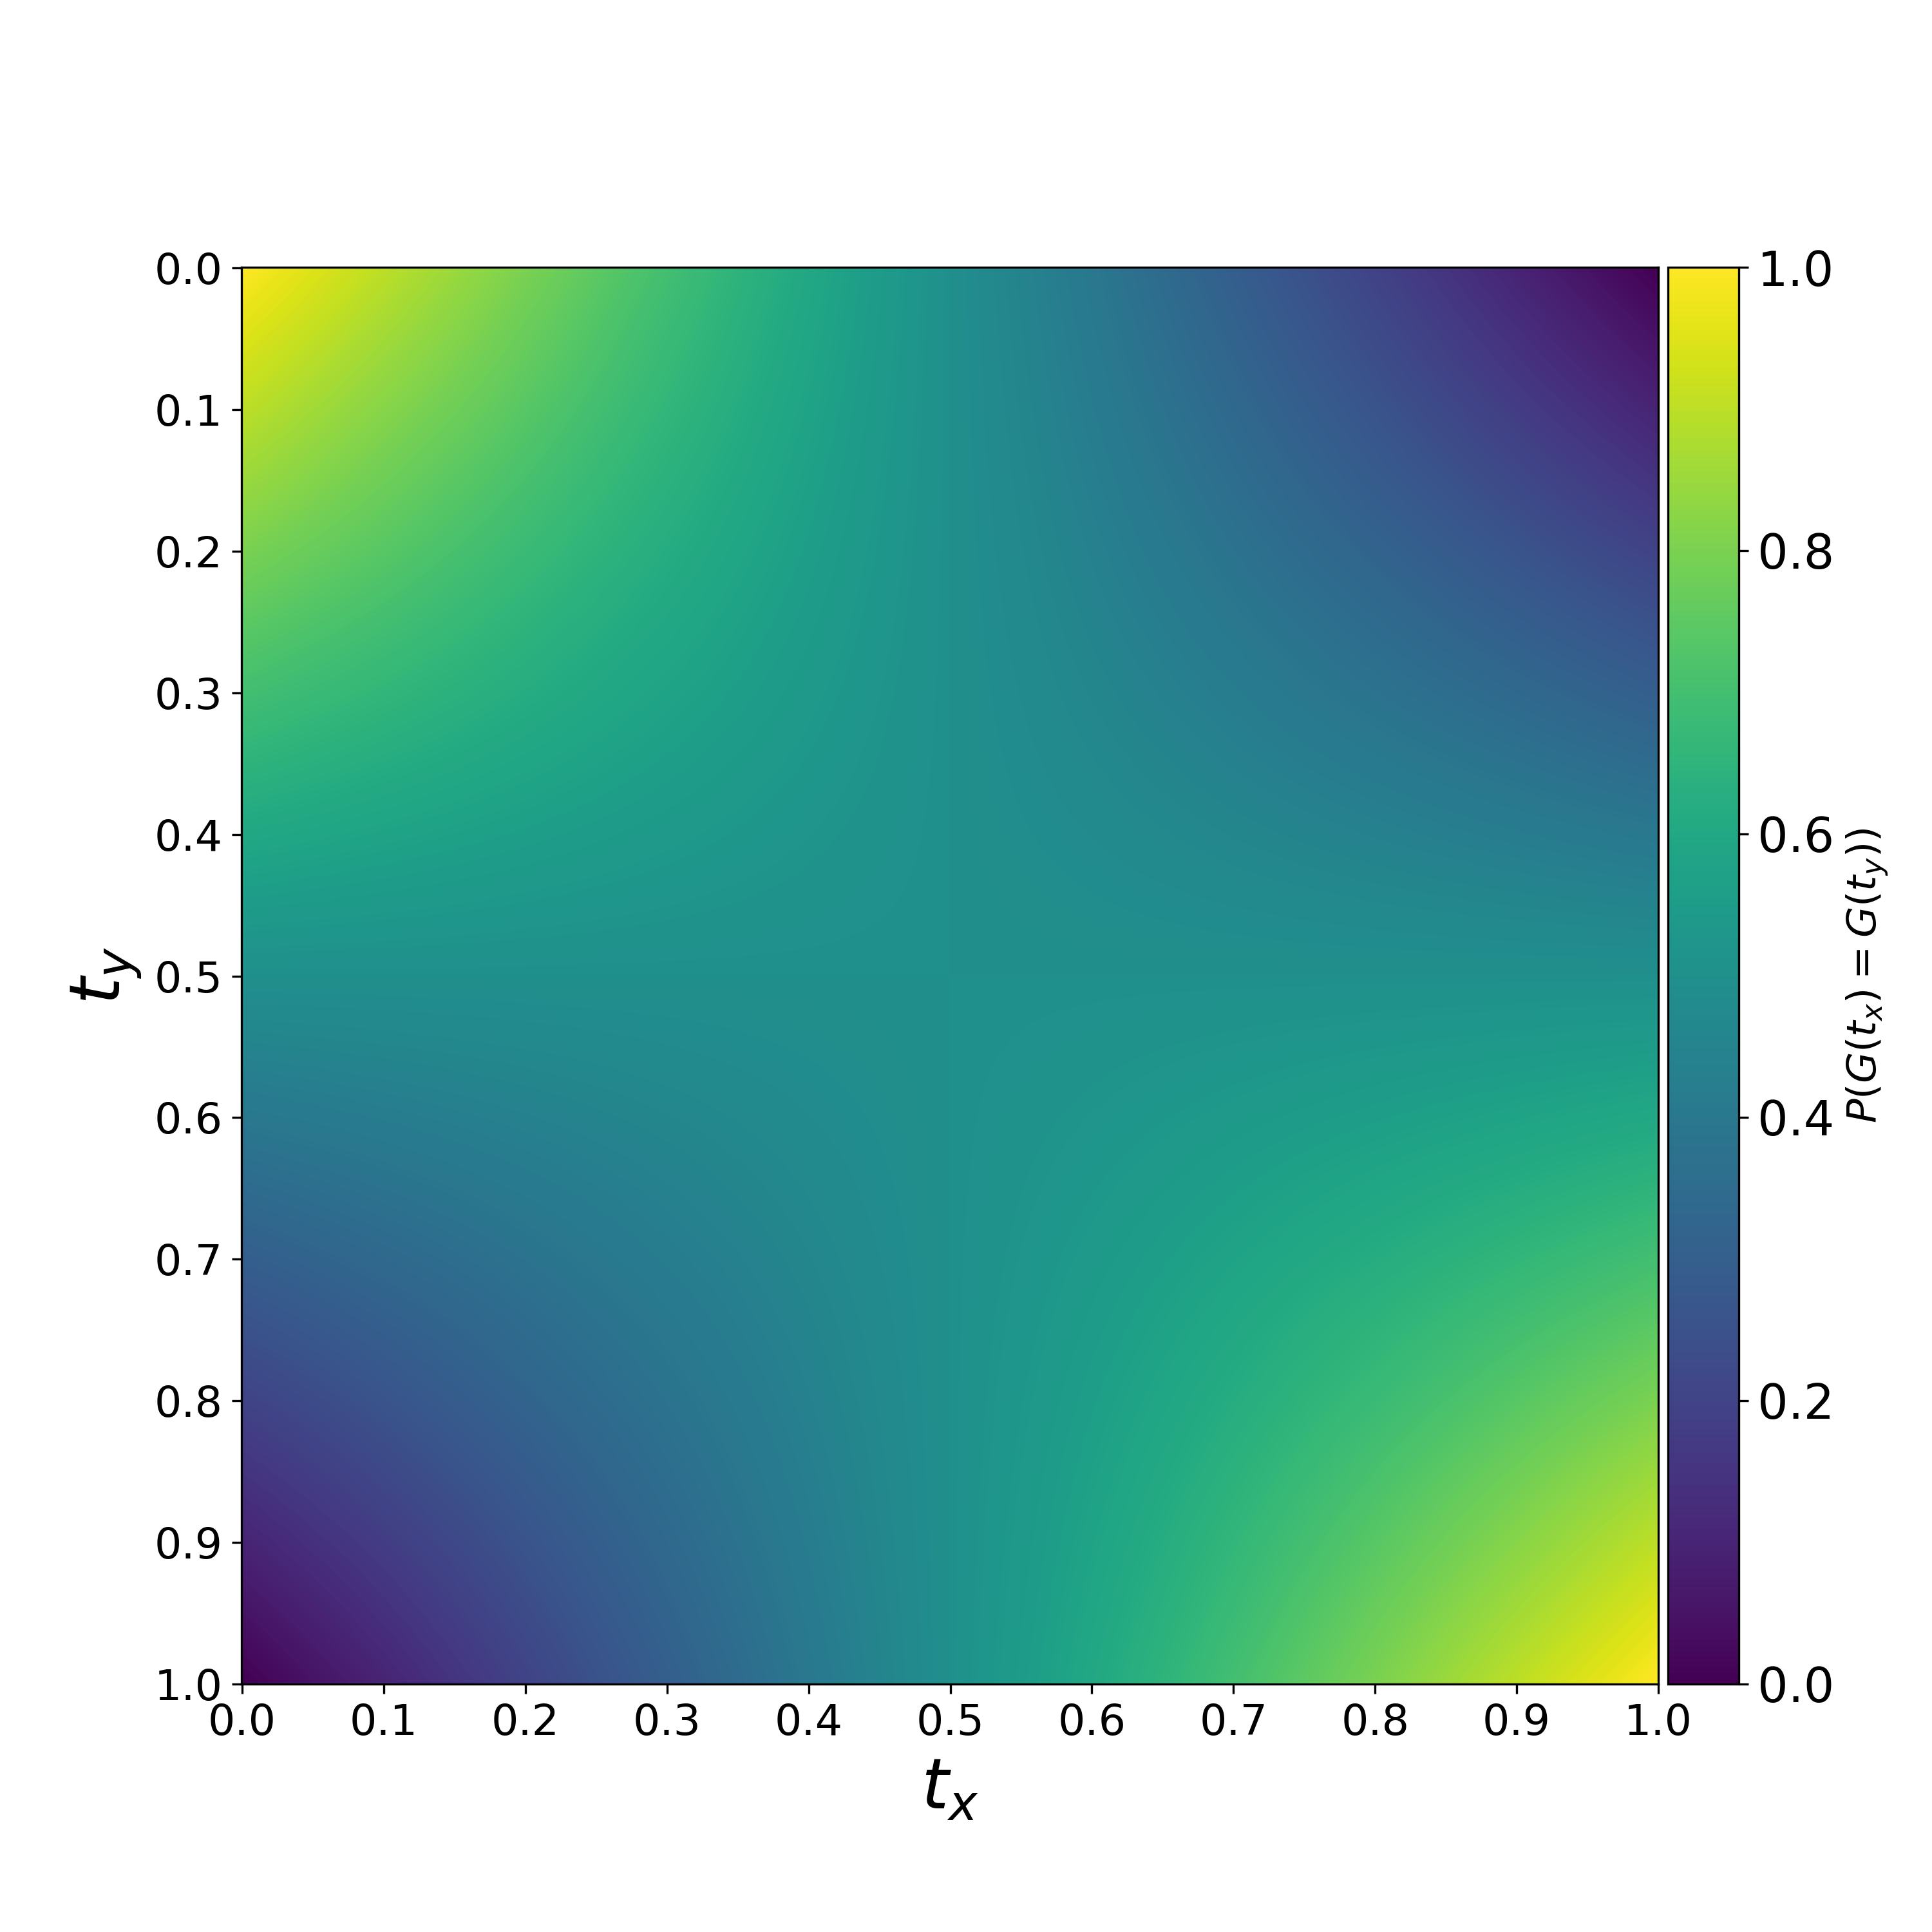
\includegraphics[width=0.5\linewidth]{ch.hourglass/images/math_inverse.png}
    \caption{\textbf{The probability of two genes being equal in a simple system displays an inverse hourglass.} This assumes a simple system of two genes (x and y) that both start in the same \textit{off} state and at a random time point switch to an \textit{on} state. }\label{fig:inverse_math}
\end{figure}

\begin{figure}[H]
    \center
    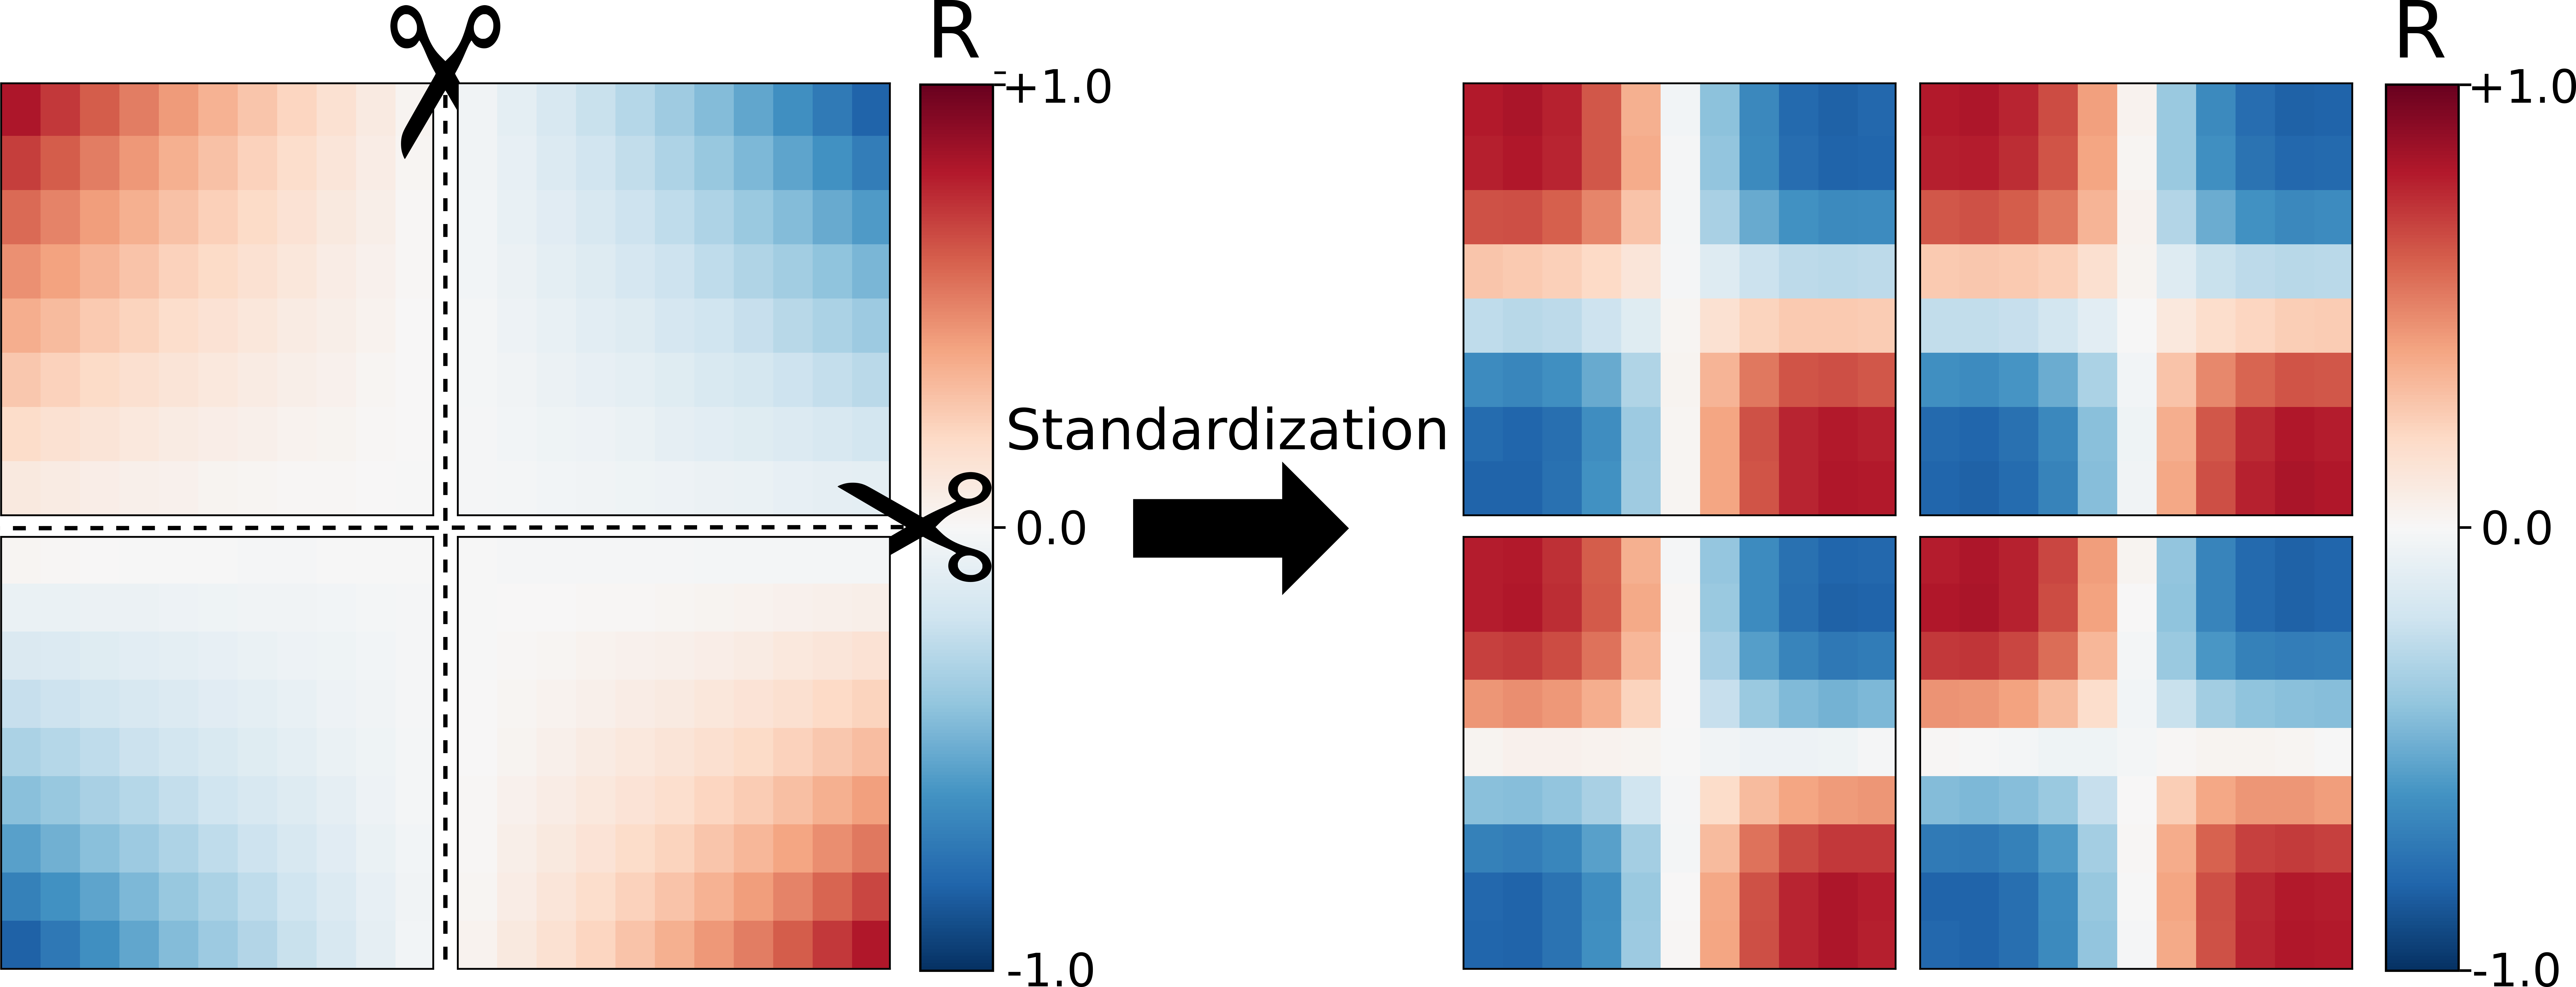
\includegraphics[width=\linewidth]{ch.hourglass/images/sim_normalisation.png}
    \caption{\textbf{Simulated data after being divided into four equal parts still shows an inverse hourglass after standardization.} This is a clear indication that the simulated suffers from the same statistical artifact as the real biological data. This means that two data sets that have no temporal relation can still show a temporal pattern.}
    \label{fig:sim_normalisation}
\end{figure}

\begin{figure}[H]
    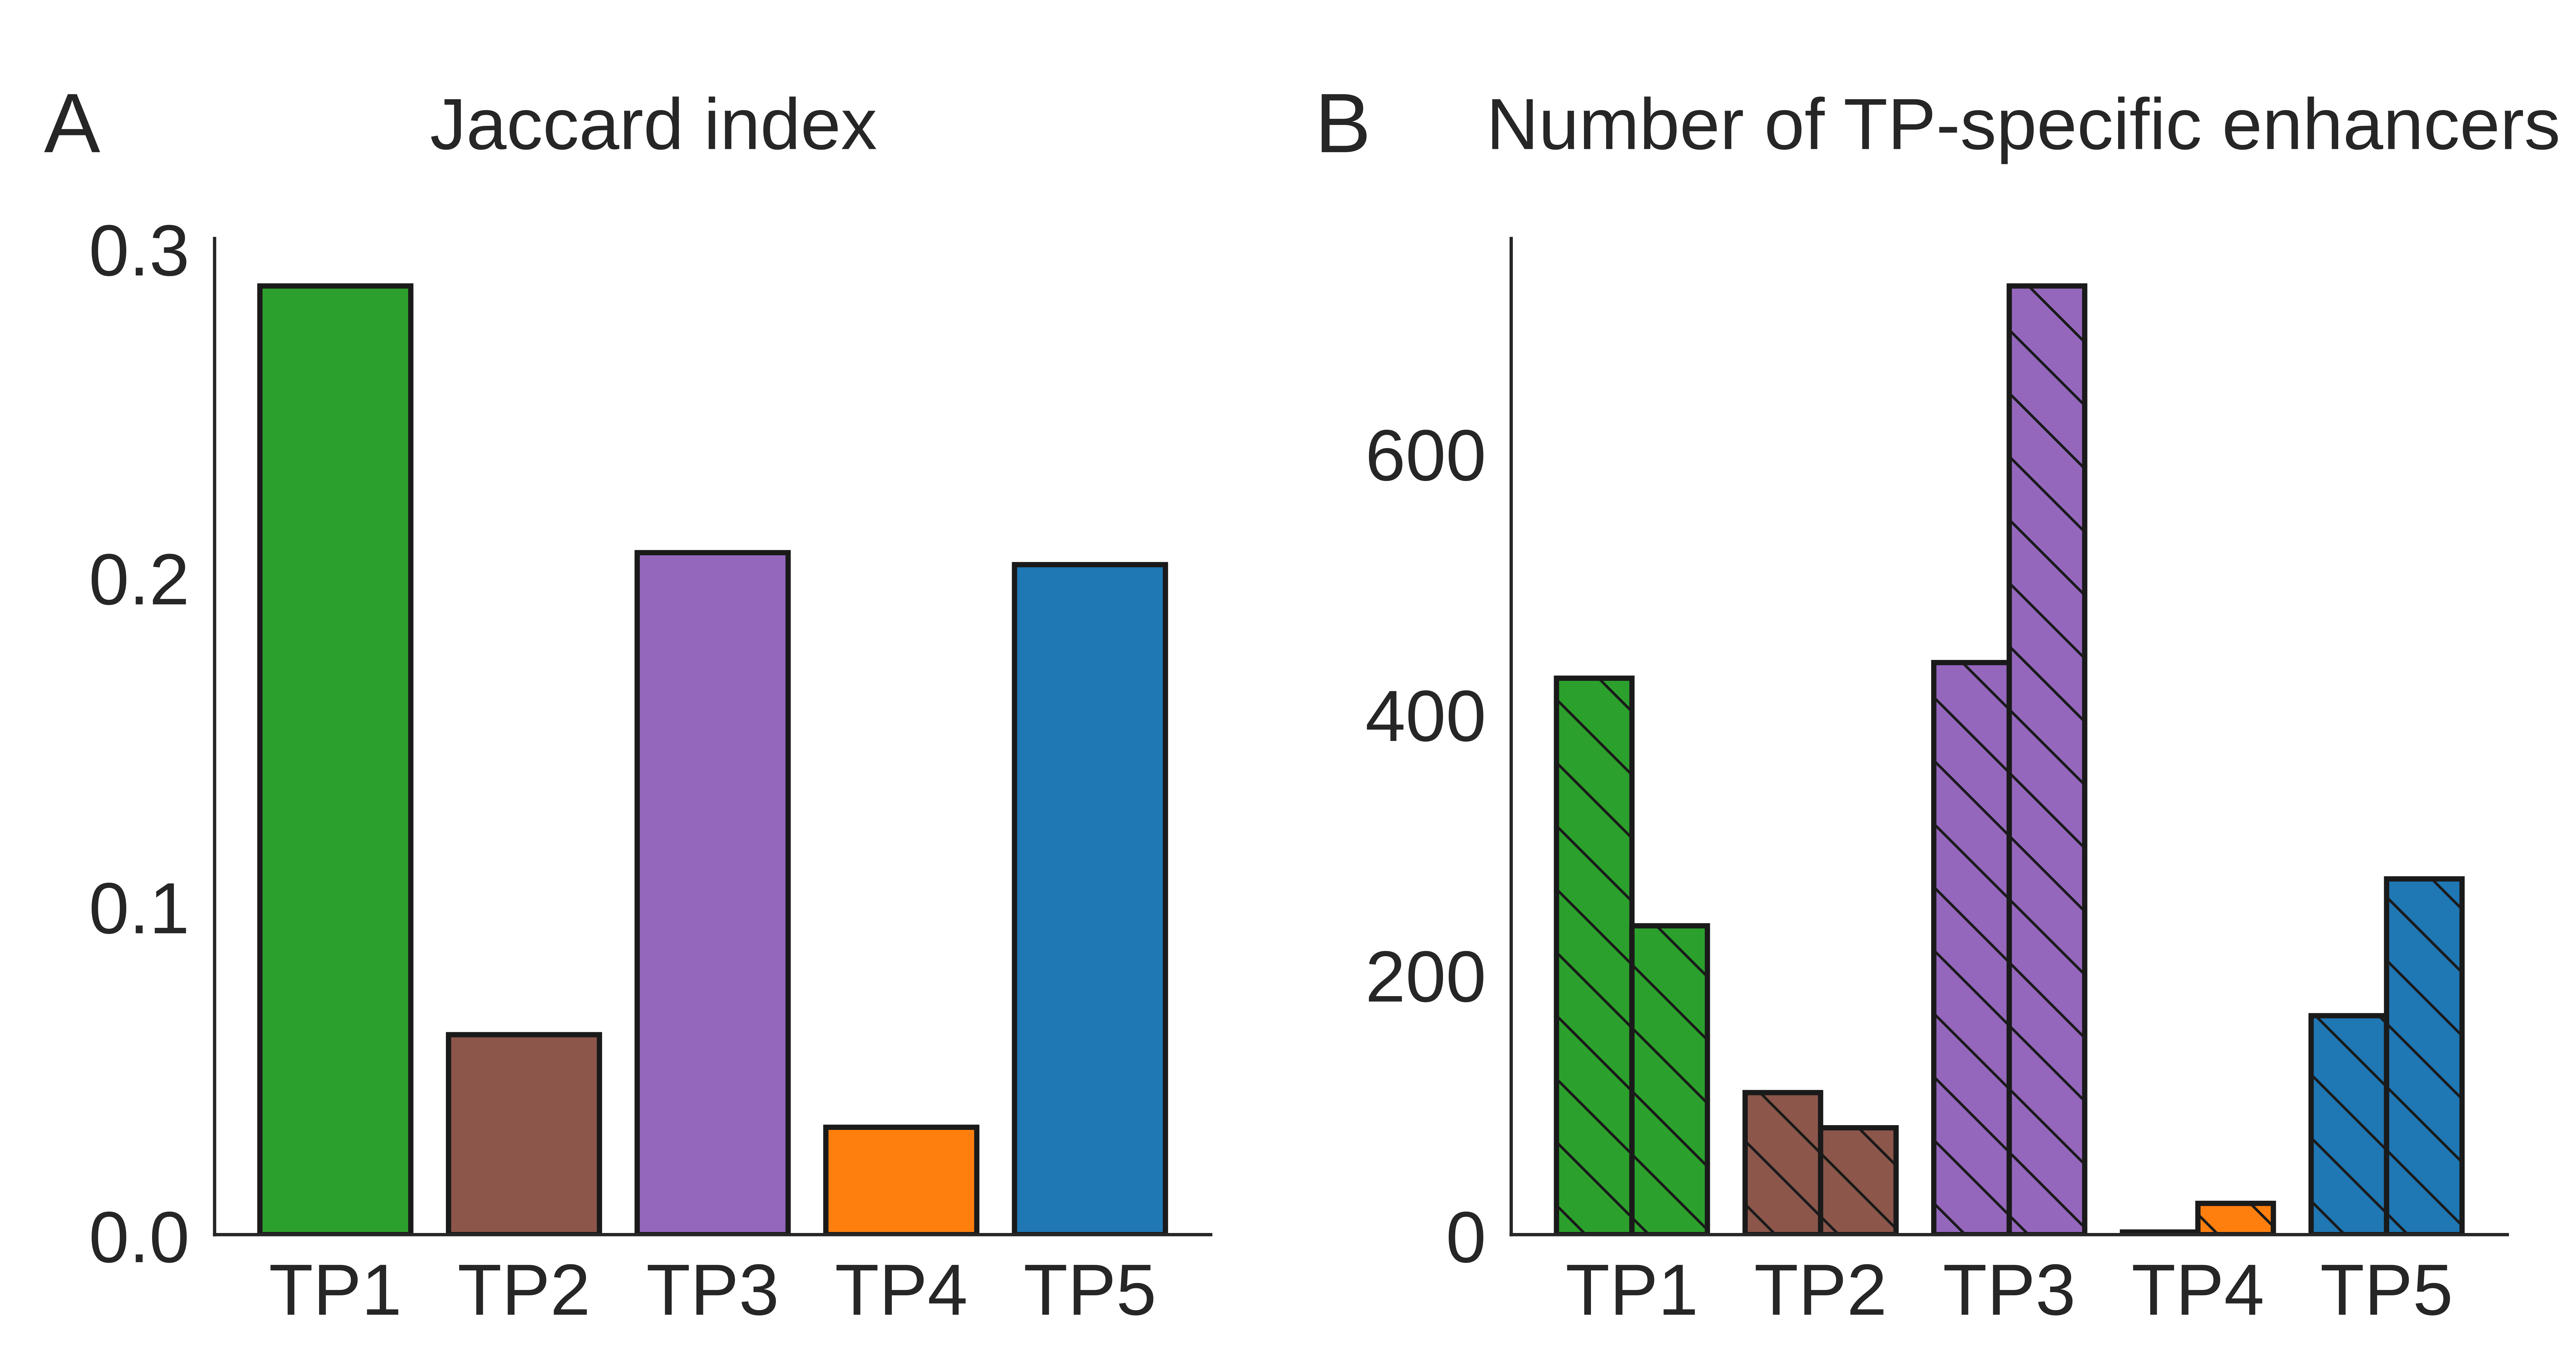
\includegraphics[width=0.9\linewidth]{ch.hourglass/images/enhancers_within.png}
    \caption{\textbf{Within species dependence of the Jaccard index on the number of enhancers}. \textbf{(A)} The proportion of conserved stage-specific enhancers at each development stage \textit{D. virilis} replicates. \textbf{(B)} The number of time-point specific enhancers for \textit{D. virilis} replicates over time. }
    \label{fig:peak_within}
\end{figure}

\begin{figure}[H]
    \center
    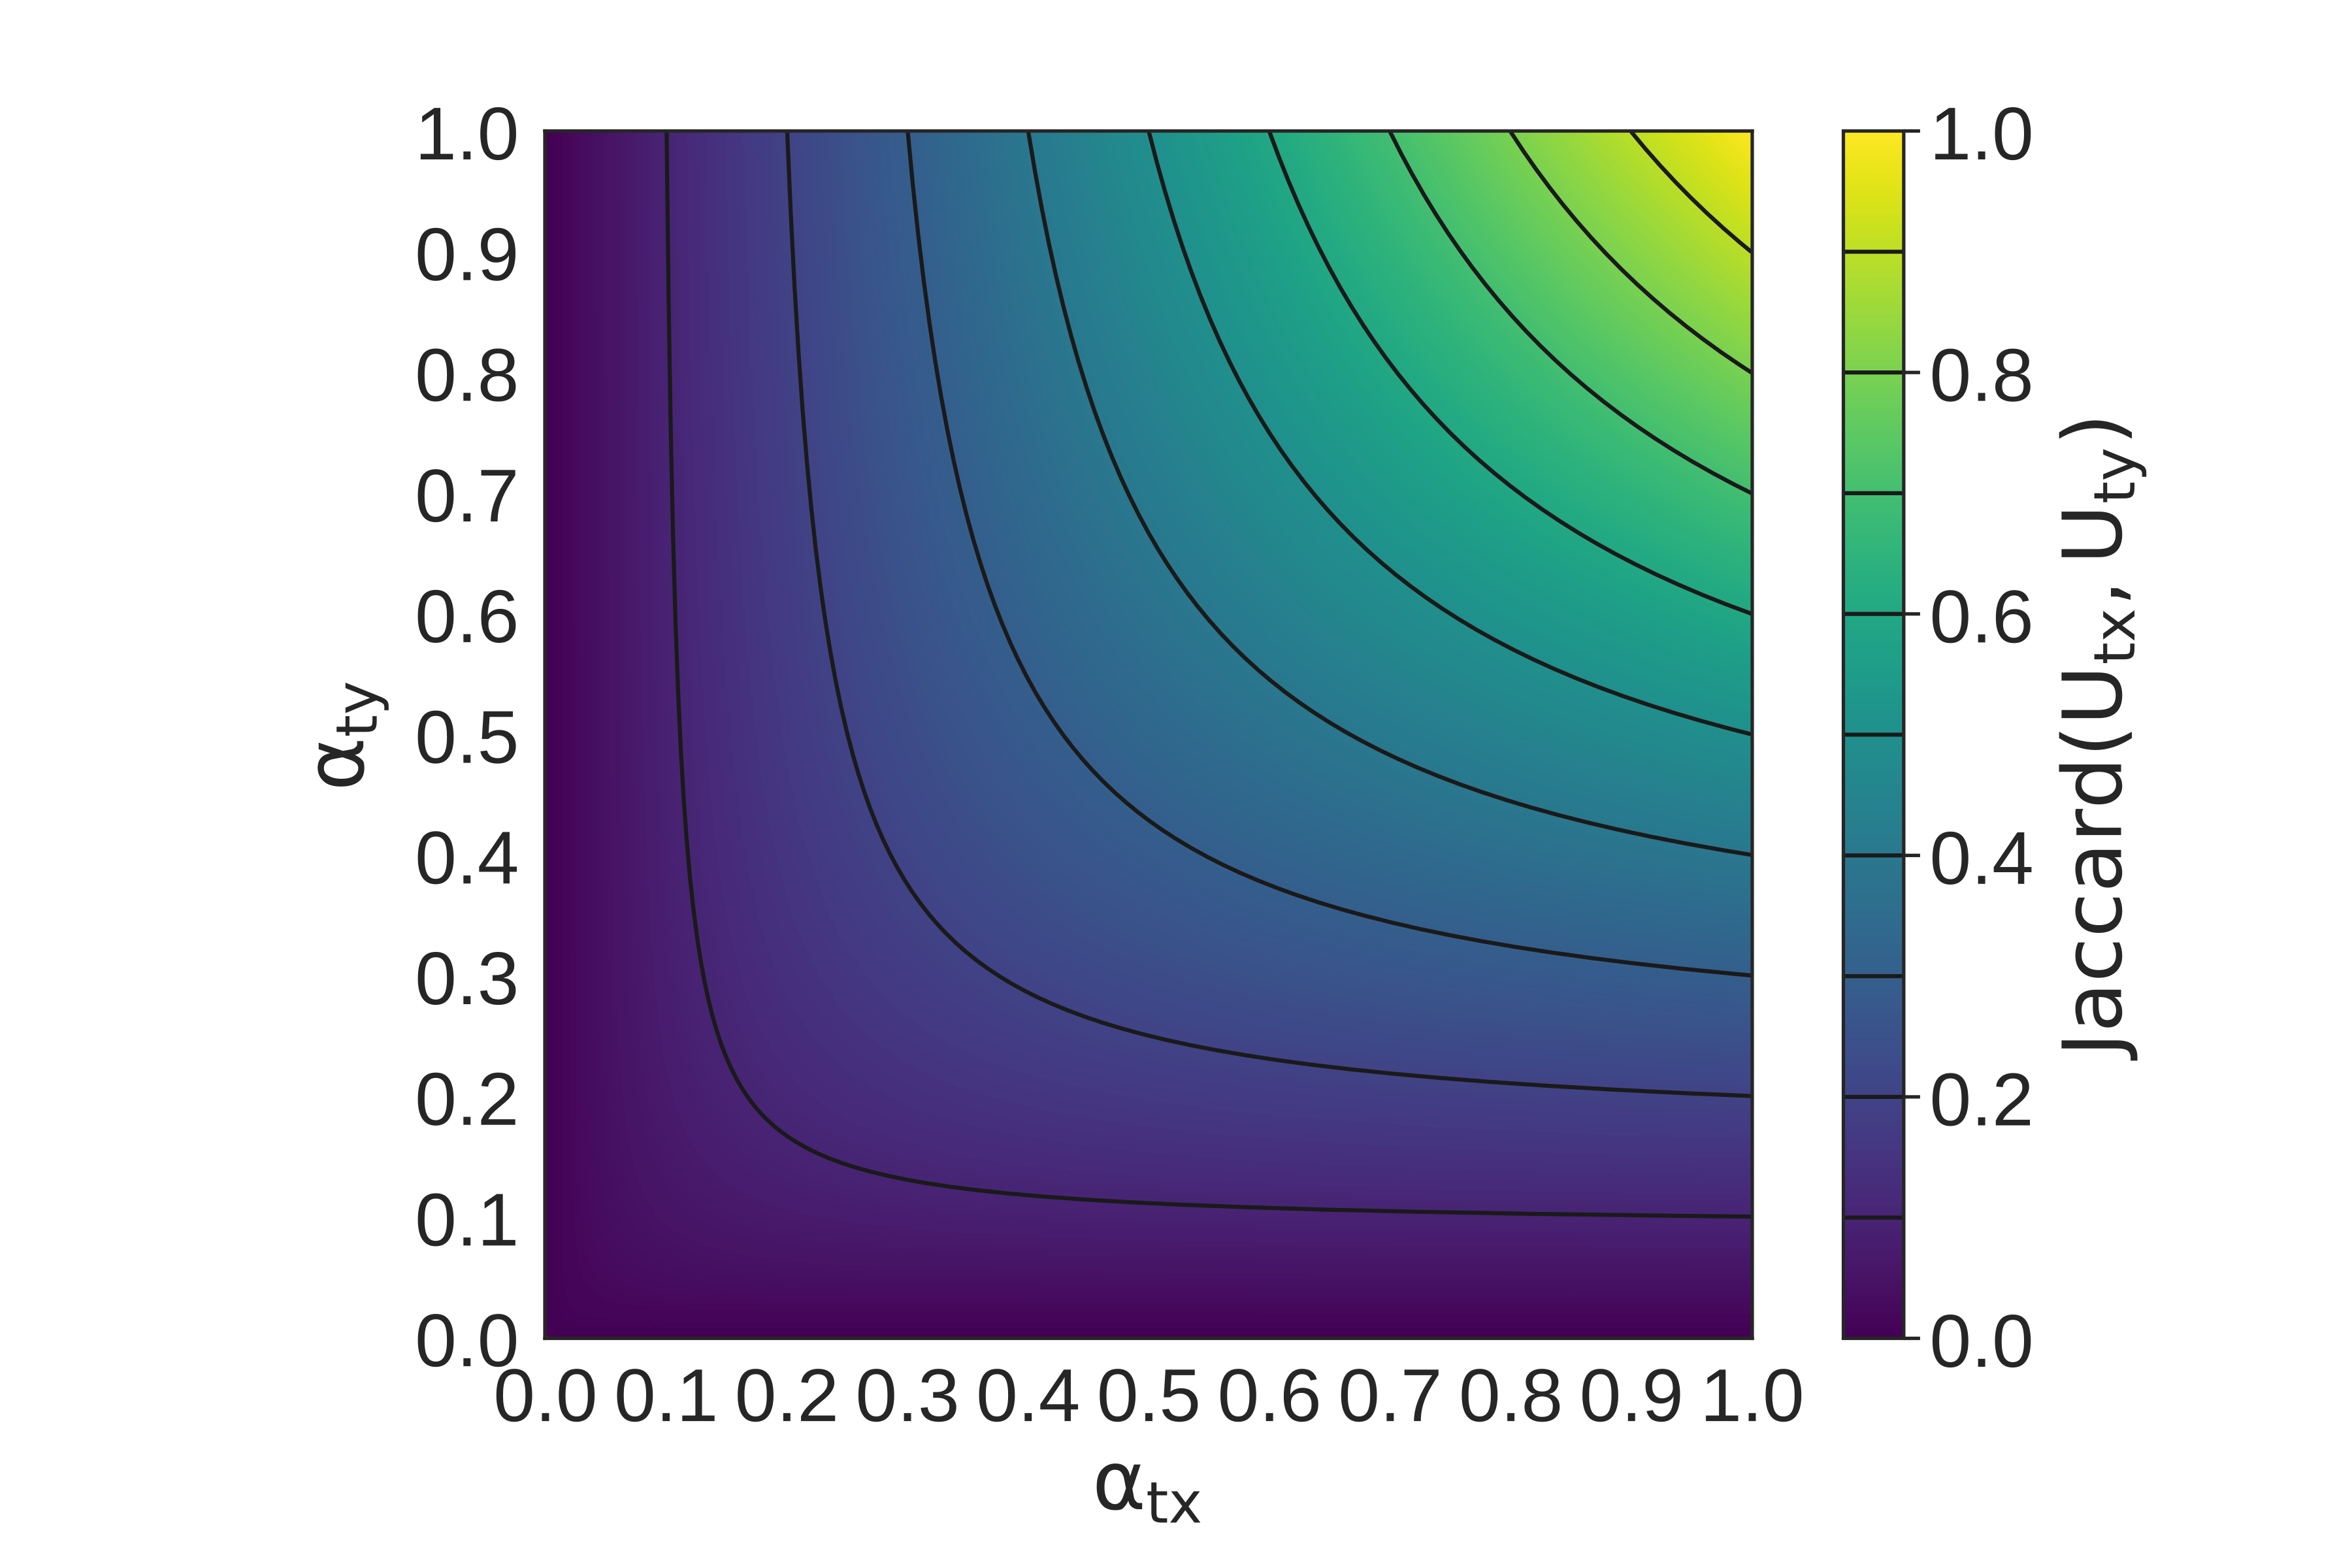
\includegraphics[width=0.7\linewidth]{ch.hourglass/images/math_flies.png}
    \caption{\textbf{The Jaccard index landscape for a different ratio of time-point specific enhancers.} This assumes that all enhancers are shared between two species, and $\alpha_{tx}$ is the ratio of total enhancers found at timepoint $t$ for species $x$. The Jaccard index depends on the number of enhancers found and is especially sensitive to the lowest number of enhancers found in the two time series. This effect is present in the real data of figure \ref{fig:peak_between} and figure \ref{fig:peak_within}. }
    \label{fig:peak_math}
\end{figure}

\begin{figure}[H]
    \center
    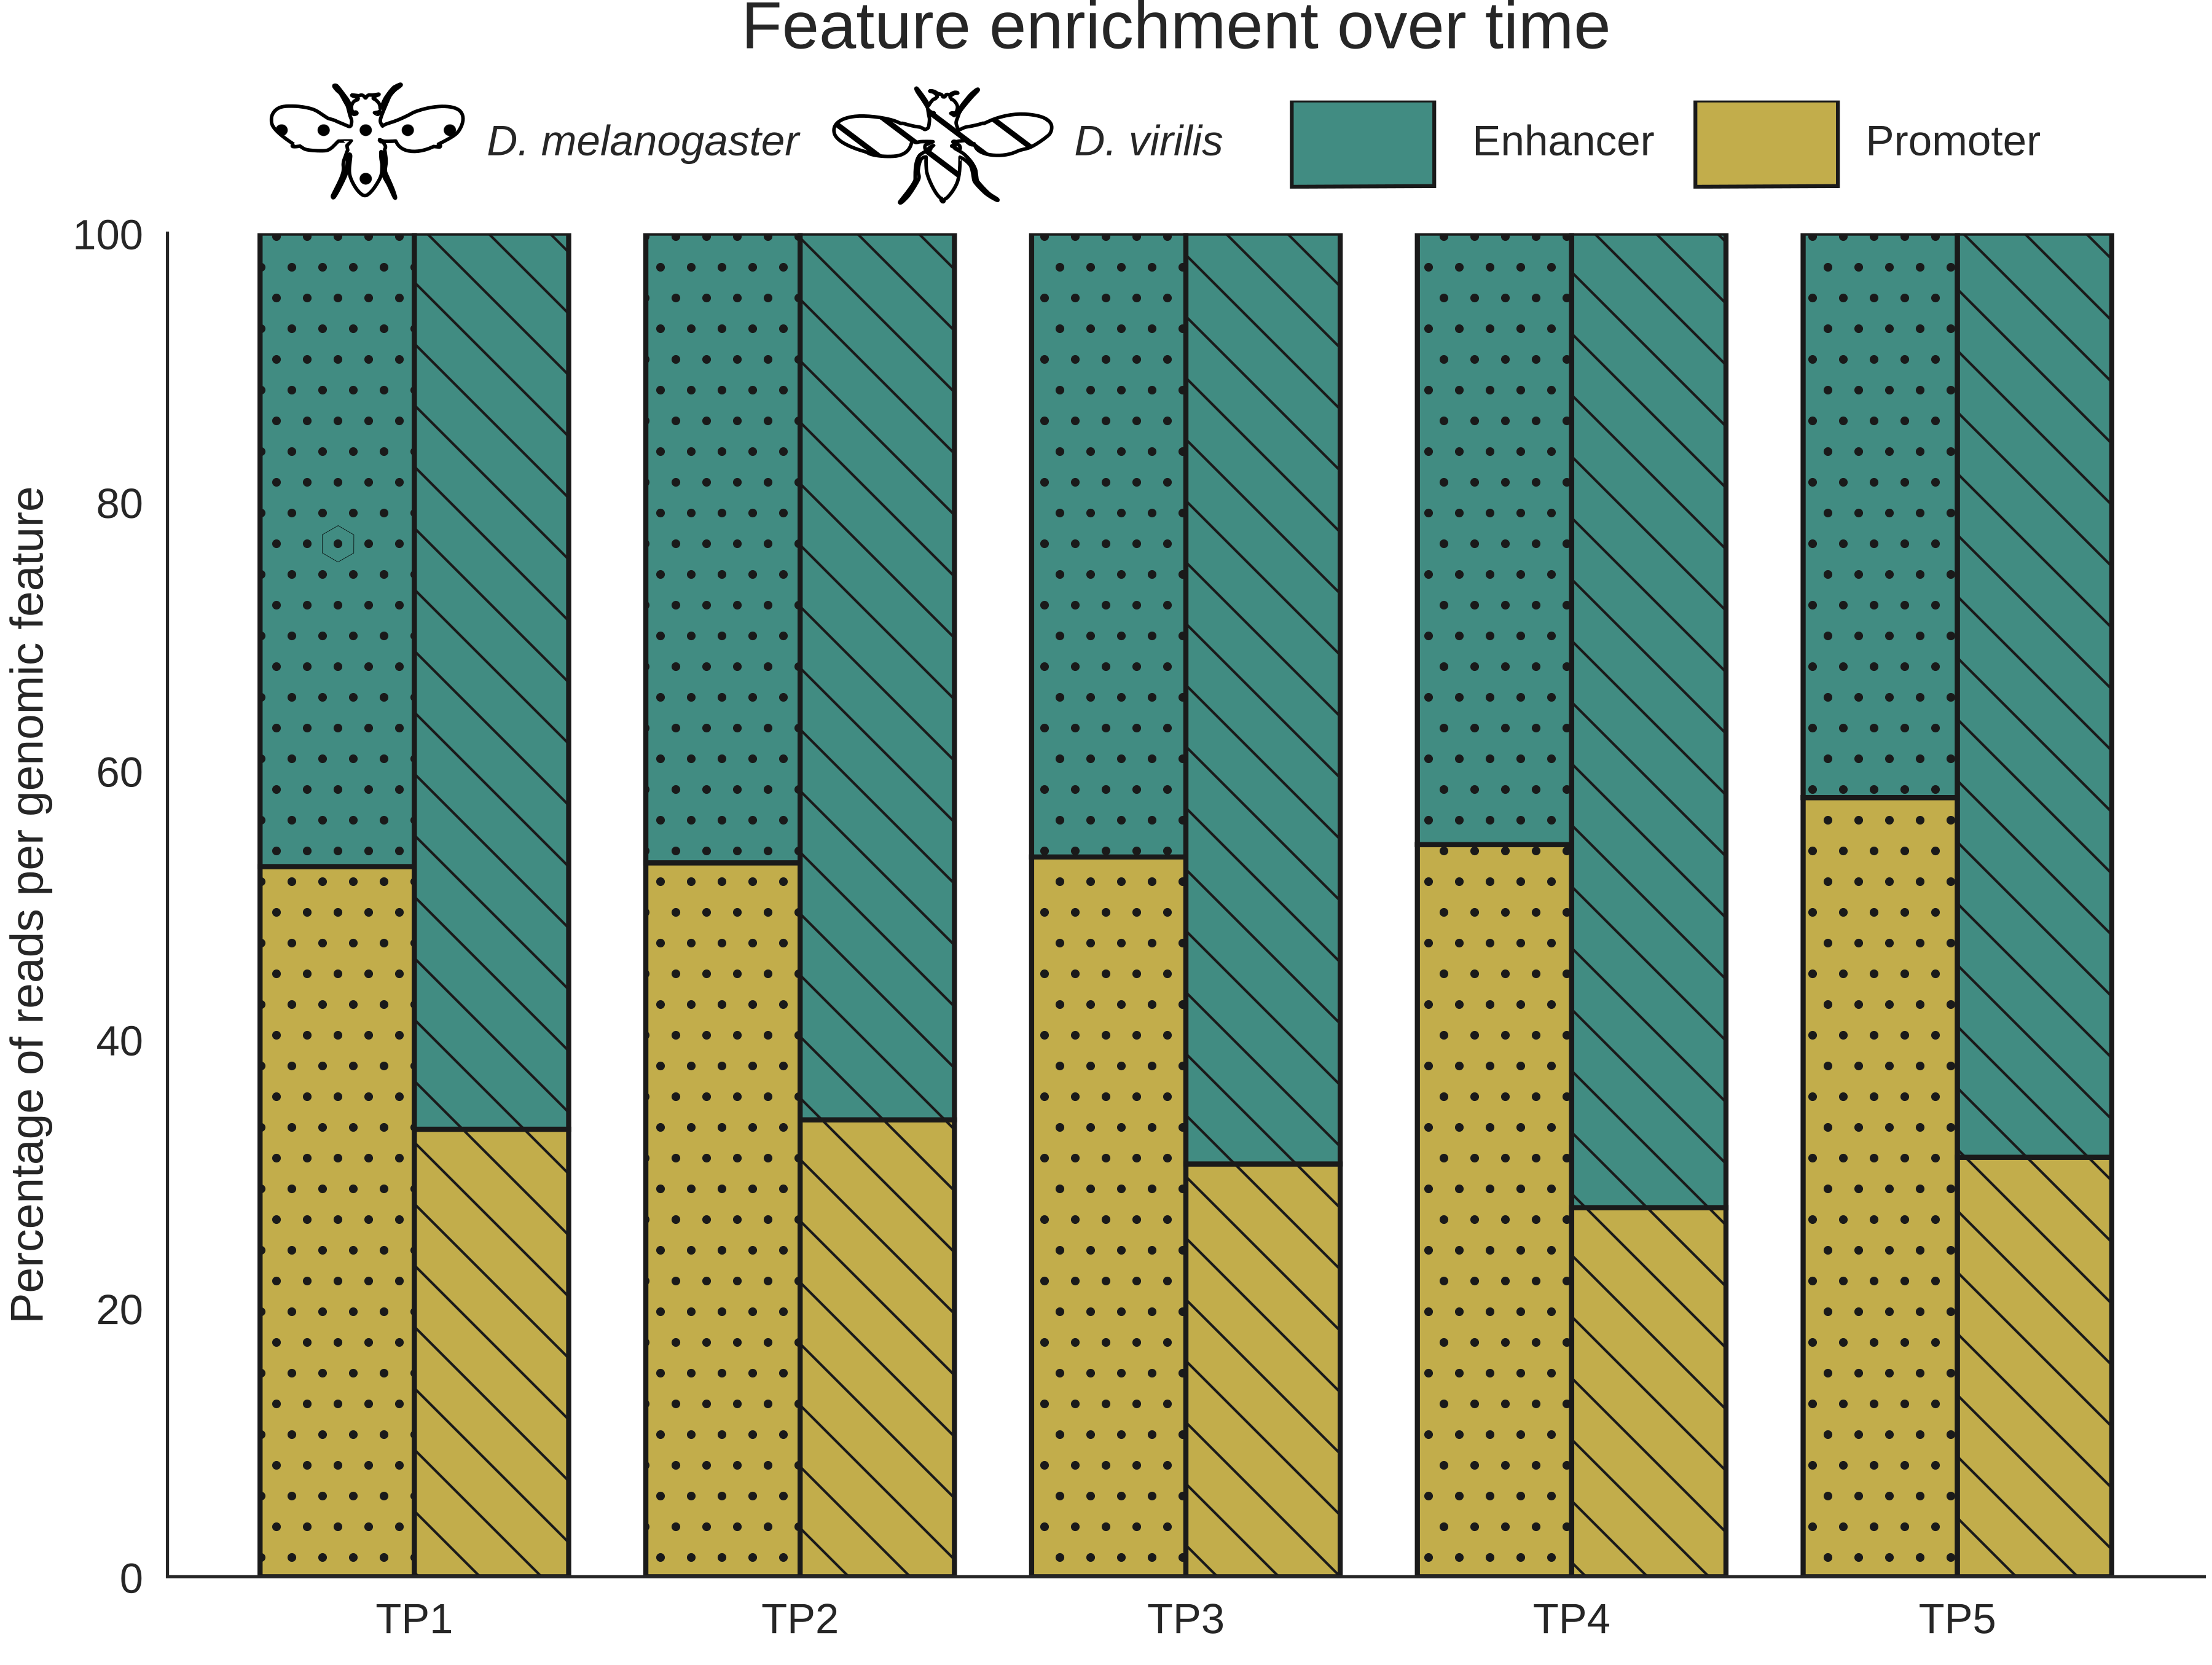
\includegraphics[width=0.8\linewidth]{ch.hourglass/images/feature_enrichment.png}
    \caption{\textbf{There are no major sudden changes in the accessibility of enhancers and promoters during \textit{Drosophila} embryonic development.} Bar plots of the percentage of reads in the consensus peak set belonging to either enhancers or promoters. Only looking at the number of enhancers per time-point can give a false indication of chance, as the total amount of peaks called can change as well as the signal-to-noise ratio.}
    \label{fig:peak_enrichment}
\end{figure}

\closesupplement
